         \chapter{Klassifikasie van Materie}\fancyfoot[LO,RE]{Chemie: Materie en Materiale}\label{chap:classification}
    \setcounter{figure}{1}
    \setcounter{subfigure}{1}
%     \label{09a7a4809656be0b739ee130746cd803}
%          \section{Mixtures, compounds and elements}
%     \nopagebreak
    \label{m38708*cid1}
\section{Materiale}
\nopagebreak

Alles wat ons in die w\^ereld rondom ons sien is gemaak van materie. Die lug wat ons inasem, die grond waarop ons loop, die kos wat ons eet, die diere en plante wat rondom ons is, bestaan uit materie. Selfs ons eie menslike liggaam is gemaak van materie!\par 
            
\begin{minipage}{.5\textwidth}
Verskillende voorwerpe kan van verskillende soorte \textbf{materiale} (stowwe) gemaak word (die materie waarvan voorwerpe gemaak word). Byvoorbeeld, 'n kas ( 'n \textsl{voorwerp}) word van hout, spykers, skarniere en knoppe (die \textsl{materiaal}) gemaak. Die \textbf{eienskappe} van die materiaal be\"invloed die eienskappe van die voorwerp. In die voorbeeld van die kas, maak die sterkte van die hout en metaal die kas sterk en duursaam. Elektriese drade word van metaal (bv. koper) gemaak omdat metale 'n tipe stof is wat kan elektrisiteit gelei. Dit is baie belangrik om die eienskappe van materiale of stowwe te verstaan sodat ons dit kan gebruik in ons huise, die industrie en op ander gebiede. In hierdie hoofstuk, sal ons kyk na verskillende soorte materiale en hulle eienskappe.\par 
\end{minipage}
\begin{minipage}{.5\textwidth}
\begin{center}
 \includegraphics[width=.8
\textwidth]{photos/cupboardby-grongar-flickr.jpg}\par
\textit{Prent verskaf deur grongar op Flickr.com}
\end{center}
\end{minipage} \\
\label{m38708*id0132}Sommige van die eienskappe van materie wat jy behoort te ken is:
\label{m38708*lid825}\begin{itemize}[noitemsep]
  \item Materiale (stowwe) kan \textbf{sterk} wees en weerstand bied teen buiging (bv. bakstene, rotse) of \textbf{swak} en maklik buigbaar (bv. klere).
  \item Materiale wat hitte gelei (bv. metale) word \textbf{termiese geleiers} genoem. Materiale wat elektrisiteit gelei (bv. koperdraad) is \textbf{elektriese geleiers}.
  \item \textbf{Bros} materiale breek maklik (bv. plastiek). Materiale wat \textbf{smeebaar} is (bv. klei, deeg), kan maklik in verskillende vorms gevorm word. Smeebare materiale kan in lang drade uitgerek word (bv. koper).
  \item \textbf{Magnetiese} materiale het 'n magnetiese veld (bv. yster).
  \item \textbf{Digtheid} is die massa per eenheid volume. By voorbeeld, klippe is digter as beton en beton is digter as modder.
  \item Die \textbf{kook- en smeltpunte} van stowwe vertel ons van die temperatuur waarteen die stof sal kook of smelt. Dit help ons om stowwe te klassifiseer as vastestowwe, vloeistowwe of gasse by 'n spesifieke temperatuur.\end{itemize}
\par 

      \label{m38708*id62556}Die diagram hieronder toon 'n manier waarvolgens materie geklassifiseer (gegroepeer) kan word volgens verskillende eienskappe. As jy verder lees in hierdie hoofstuk, sal jy sien dat daar ook ander maniere van die klassifikasie van stowwe is, byvoorbeeld of die stof 'n goeie elektriese geleier is of nie.\par 
    \setcounter{subfigure}{0}
	\begin{figure}[H] % horizontal\label{m38708*uid1}
    \begin{center}
\scalebox{.8}{
\begin{pspicture}(-6,0.5)(6,5)
%\psgrid[gridcolor=lightgray]
\rput(0,4.8){\textbf{MATERIE}}
\psline(-3,4)(-3,4.4)(3,4.4)(3,4)
\rput(-3,3.8){\textbf{MENGSELS}}
\rput(3,3.8){\textbf{SUIWER  STOWWE}}
\psline(-3,3.4)(-3,3.6)
\psline(3,3.4)(3,3.6)
\psline(-4.5,3)(-4.5,3.4)(-1.5,3.4)(-1.5,3)
\psline(4.5,3)(4.5,3.4)(1.5,3.4)(1.5,3)
\rput(-4.5,2.8){Homogene}
\rput(-1.5,2.8){Heterogene}
\rput(4.5,2.8){Verbindings}
\rput(1.5,2.8){Elemente}
\psline(1.5,2.6)(1.5,2.4)
\psline(0,2.0)(0,2.4)(3,2.4)(3,2.0)
\rput(0,1.8){Metale}
\rput(3,1.8){Nie-metale}
\psline(0,1.4)(0,1.6)
\psline(-1.5,1.2)(-1.5,1.4)(1.5,1.4)(1.5,1.2)
\rput(-1.5,1){Magneties}
\rput(1.5,1){Nie-magneties}
%\psset{yunit=0.5}
\end{pspicture}
}
    \end{center}
\caption{Klassifikasie van materie.}
\label{fig:c:ClassificationOfMatter}
 \end{figure}      
    \label{m38708*eip-344}\begin{activity}{Uit watter stowwe word produkte gemaak?}
{
\begin{minipage}{.5\textwidth}
Hierdie aktiwiteit let op die stowwe waaruit voedselprodukte saamgestel is. In groepe van 3 of 4 kyk na die etikette op kositems. Maak 'n lys van die bestanddele. Kan jy (deur na die bestanddele te kyk) s\^e watter kos dit is (d.w.s. speserye, olie, lekkers, ens.)? Voedselprodukte word gemerk om vir jou as verbruiker te help om te weet wat jy eet asook met die keuse van gesonder alternatiewe. Sommige kunsmatige smaakmiddels en kleurmiddels, soos mononatrium glutamaat (MSG van die Engels ``Monosodium Glutamate'') en tartrasien word deesdae minder in kosse gebruik vir gesondheidsredes. Is daar ander bestanddele in die produkte wat onveilig is om te eet? Watter preserveermiddels en byvoegings (bv. tartrasien, MSG, kleurmiddels) is daar? Is hierdie preserveermiddels en byvoegings goed vir jou? Is daar natuurlike (van plante afkomstig) alternatiewe? Wat gebruik verskillende inheemse groepe mense om hulle kos te geur en te bewaar?
\end{minipage}
\begin{minipage}{.5\textwidth}
 \begin{center}
 \includegraphics[width=.8\textwidth]{photos/food_labels.png}\par
\end{center}
\end{minipage}

 }  \end{activity}
\begin{activity}{Klassifiseer stowwe} {
\begin{minipage}{.4\textwidth}
Kyk rondom jou na verskillende strukture. Maak 'n lys van al die verskillende materiale wat jy sien. Probeer om uit te werk waarom 'n spesifieke materiaal gebruik is. Kan jy al die verskillende materiale wat gebruik is volgens hul eienskappe klassifiseer? Waarom is hierdie materiale bo ander materiale gekies?
\end{minipage}
\begin{minipage}{.3\textwidth}
\begin{center}
 \includegraphics[height=.7\textwidth]{photos/windmillby-flowcomm-flickr.jpg}\par
\textit{Prent verskaf deur flowcomm op Flickr.com}
\end{center}
\end{minipage}
\begin{minipage}{.3\textwidth}
\begin{center}
 \includegraphics[height=.7\textwidth]{photos/materials.png}\par
\end{center}
\end{minipage}
}
\end{activity}


\label{m38708*cid2}
            \section{Mengsels}
            \nopagebreak
            \label{m38708*id62584}Ons sien die hele tyd mengsels in ons alledaaglikse lewe. 'n Bredie is, byvoorbeeld, 'n mengsel van verskillende voedselsoorte soos vleis en groente, seewater is 'n mengsel van water, sout en ander stowwe, en die lug is 'n mengsel van gasse soos koolstofdioksied, suurstof en stikstof.\par 
\label{m38708*fhsst!!!underscore!!!id69}
\Definition{\label{id2405672}Mengsel} {\label{m38708*meaningfhsst!!!underscore!!!id69}
      'n Mengsel word uit twee of meer stowwe saamgestel. Hierdie stowwe is nie verbind of aanmekaar geheg nie en geen chemiese reaksie het plaasgevind nie.
       } 
      \label{m38708*id62612}Die stowwe waaruit die mengsel bestaan:\par 
      \label{m38708*id62615}\begin{itemize}[noitemsep]
            \label{m38708*uid2}\item \textbf{word nie in 'n vaste verhouding gemeng nie.} \\
Verbeel jou jy het 250 ml water en jy voeg sand by die water. Dit maak nie saak of jy 20 g, 40 g, 100 g of enige ander massa sand by die water voeg nie, dit sal steeds 'n mengsel van sand en water wees.
\label{m38708*uid3}\item \textbf{behou hul fisiese eienskappe.} \\
In die voorbeeld wat ons gebruik het, het nie een van die stowwe op enige manier verander toe hulle saam gemeng is nie. Die sand is nog sand en die water is nogsteeds water.
\label{m38708*uid4}\item \textbf{kan op 'n meganiese wyse geskei word.} \\
Om iets volgens ``meganiese wyse'' te skei, beteken dat daar geen chemiese proses betrokke was nie. In ons sand en water voorbeeld, is dit moontlik om die mengsel te skei deur eenvoudig die water deur 'n filter te giet. Iets \textsl{fisies} word met die mengsel gedoen, eerder as iets \textsl{chemies}.
\end{itemize}
      \label{m38708*id62700}Ons kan mengsels verder in twee hoofgroepe verdeel naamlik: heterogeen en homogeen.\par 

      \label{m38708*uid5}
            \subsection*{Heterogene Mengsels}
            \nopagebreak
        \label{m38708*id62715} 'n \textbf{Heterogene} mengsel het nie 'n definitiewe samestelling nie. Ontbytgraan in melk is 'n voorbeeld van 'n heterogene mengsel. Grond is nog 'n voorbeeld. Grond het klippies, plantmateriaal en sand in. Alhoewel jy een stof by 'n ander stof voeg, bly hulle afsonderlik in die mengsel. Ons s\^e heterogene mengsels is \textsl{nie-uniform}, met ander woorde hulle is nie presies dieselfde regdeur nie.\par 
\begin{minipage}{.5\textwidth}
\begin{center}
 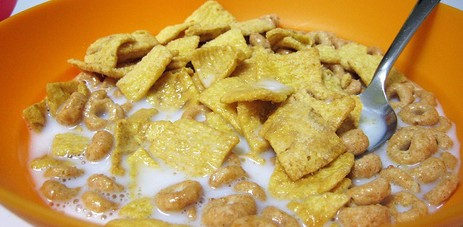
\includegraphics[width=.8\textwidth]{photos/mixtureby-dougww-flickr.jpg}\par
\textit{Prent verskaf deur dougww op Flickr.com}
\end{center}
\end{minipage}
\begin{minipage}{.5\textwidth}
\begin{figure}[H]
\label{fig:heterogeneousmixture}
\begin{center}
 \begin{pspicture}(0,-1)(11,4.7)
\SpecialCoor
\psframe[fillstyle=crosshatch*,fillcolor=white,hatchcolor=lightgray,hatchwidth=1.2pt,hatchsep=1.8pt,hatchangle=0](0,0)(4,4)
\pscircle[fillcolor=lightgray,fillstyle=solid](0.5,0.5){0.2}
\pscircle[fillcolor=white,fillstyle=solid](1,1.2){0.1}
\pscircle[fillcolor=lightgray,fillstyle=solid](2.1,1){0.2}
\pscircle[fillcolor=white,fillstyle=solid](2.3,0.4){0.1}
\pscircle[fillcolor=lightgray,fillstyle=solid](3.5,1){0.2}
\pscircle[fillcolor=white,fillstyle=solid](0.5,1.6){0.1}
\pscircle[fillcolor=white,fillstyle=solid](1,2){0.1}
\pscircle[fillcolor=white,fillstyle=solid](1.8,1.5){0.1}
\pscircle[fillcolor=lightgray,fillstyle=solid](2,2){0.2}
\pscircle[fillcolor=lightgray,fillstyle=solid](0.5,2.7){0.2}
\pscircle[fillcolor=lightgray,fillstyle=solid](2.3,2.5){0.2}
\pscircle[fillcolor=white,fillstyle=solid](2.5,2.8){0.1}
\pscircle[fillcolor=white,fillstyle=solid](3,3){0.1}
\pscircle[fillcolor=white,fillstyle=solid](3.5,2.4){0.1}
\pscircle[fillcolor=white,fillstyle=solid](0.5,3.5){0.1}
\pscircle[fillcolor=white,fillstyle=solid](2,3.4){0.1}
\pscircle[fillcolor=lightgray,fillstyle=solid](3.5,3.5){0.2}
\pscircle[fillcolor=lightgray,fillstyle=solid](1.7,3.1){0.2}
\pscircle[fillcolor=white,fillstyle=solid](3,3){0.1}
\end{pspicture}
\end{center}
\caption{ 'n Submikroskopiese voorstelling van 'n heterogene mengsel. Die grys sirkels stel een stof (bv. 'n ontbytgraan) voor en die wit sirkels stel nog 'n stof (bv. 'n ander ontbytgraan) voor. Die agtergrond is die melk.}
\end{figure}
\end{minipage}


\label{m38708*fhsst!!!underscore!!!id89}\Definition{\label{id2405839} { Heterogene mengsel }} 
{ \label{m38708*meaningfhsst!!!underscore!!!id89}
        'n Heterogene mengsel is een wat bestaan uit twee of meer stowwe, is nie-uniform en die verskillende komponente van die mengsel kan gesien word.
         } 
Heterogene mengsels kan verder onderverdeel word na gelang daarvan of dit twee vloeistowwe is wat gemeng is, 'n vaste stof en 'n vloeistof of 'n vloeistof en 'n gas of selfs 'n gas en 'n vaste stof. Vir hierdie mengsels is spesiale name gegee soos jy in die tabel hieronder sien.   \par
\begin{table}[h!]
 \begin{center}
  \begin{tabular}{|l|l|l|}\hline
   \textbf{Fases van materie} & \textbf{Naam van mengsel} & \textbf{Voorbeeld} \\ \hline
   vloeistof-vloeistof & emulsie & olie en water \\ \hline
   vaste stof-vloeistof & suspensie & modderige \\ \hline
   gas-vloeistof & a\"erosol & bruisdrankies \\ \hline
   gas-vastestof & rook & rookmis \\ \hline
  \end{tabular}

 \end{center}
\caption{Voorbeelde van verskillende heterogene mengsels}
\label{tab:mixtures}
\end{table}

      \label{m38708*uid6}
            \subsection*{Homogene mengsels}
            \nopagebreak
        \label{m38708*id62762} 'n \textbf{Homogene} mengsel het 'n definitiewe samestelling en spesifieke eienskappe. In 'n homogene mengsel kan die verskillende dele nie gesien word nie. 'n Oplossing van sout in water is 'n voorbeeld van 'n homogene mengsel. Wanneer die sout oplos, versprei dit eweredig deur die water sodat alle dele van die oplossing dieselfde is, jy kan nie meer die sout geskei van die water sien nie. Dink ook aan koffie sonder melk. Die lug wat ons inasem, is nog 'n voorbeeld van 'n homogene mengsel, want dit bestaan uit verskillende gasse wat in 'n konstante verhouding gemeng is, wat nie visueel van mekaar onderskei kan word nie (d.w.s. jy kan nie die verskillende komponente sien nie).\par 

\mindsetvid{the dissolving process}{VPabz}

\begin{minipage}{.5\textwidth}
\begin{center}
 \includegraphics[width=.3\textwidth]{photos/coffeeby_JuliusSchorzman_wikimedia.jpg}\par
\textit{Prent verskaf deur Julius Schorzman op wikimedia}
\end{center}
\end{minipage}
\begin{minipage}{.5\textwidth}
\begin{center}
 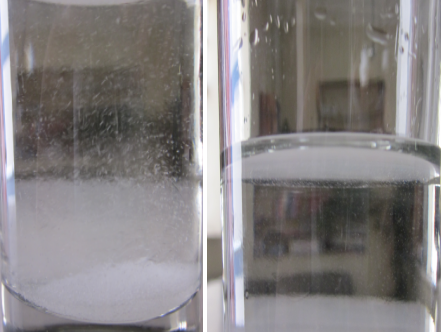
\includegraphics[width=.5\textwidth]{photos/saltwater.png}\par
\end{center}
\end{minipage}
\label{m38708*fhsst!!!underscore!!!id96}\Definition{   \label{id2405912}Homogene mengsel} { \label{m38708*meaningfhsst!!!underscore!!!id96}
        'n Homogene mengsel is een wat uniform (eenvormig) is, en waar die verskillende komponente van die mengsel nie gesien kan word nie.
         } 
%         \label{m38708*id62795}An \textbf{alloy} is a homogeneous mixture of two or more elements, at least one of which is a metal, where the resulting material has metallic properties. Alloys are usually made to improve the properties of the elements that make them up. For example steel is much stronger than iron (which is the main component of steel). Steel is a mixture (alloy) of mainly iron with carbon (to make it harder), manganese (to make it strong) and chromium (to prevent rusting).\par 

\label{m38708*eip-479}
      \begin{wex}{Mengsels}
{Vir elk van die volgende mengsels sê of dit 'n homogene of 'n heterogene mengsel is:
\label{m38708*eip-id1167649056231}\begin{enumerate}[noitemsep, label=\textbf{\alph*}. ] 
            \leftskip=20pt\rightskip=\leftskip\item suiker opgelos in water
\item koekmeel en ystervylsels (klein stukkies yster)
\item koekmeel en bakpoeier
\item smarties, jellie tots en pepermente\end{enumerate} }
%  \par 
%\vspace{5pt}
%\label{m38708*eip-602}\noindent\textbf{Solution to Exercise }
%\label{m38708*eip-id7325184}
{\westep{Kyk na die definisie}
Ons kyk eers na die definisie van 'n heterogene en homogene mengsel.
\westep{Besluit of jy die komponente kan sien of nie.}
\begin{enumerate}[noitemsep, label=\textbf{\alph*}. ] 
 %           \leftskip=20pt\rightskip=\leftskip
\item Ons kan nie die suiker in die water sien nie.
\item Ons is in staat om stukkies yster in die koekmeel te sien.
\item Daar is geen manier om te onderskei tussen die koekmeel en bakpoeier nie.
\item Ons kan duidelik elk van die komponente waaruit die mengsel bestaan, sien. \end{enumerate}
\westep{Besluit of die komponente eenvormig gemeng is of nie}
\begin{enumerate}[noitemsep, label=\textbf{\alph*}. ] 
 %           \leftskip=20pt\rightskip=\leftskip
\item Die twee komponente is eenvormig gemeng.
\item In hierdie mengsel mag daar plekke wees daar baie ystervylsels is en plekke waar daar meer koekmeel is, dus is dit nie eenvormig gemeng nie.
\item Die twee komponente van die mengsel is eenvormig gemeng.
\item Die drie komponente van die mengsel is nie eweredig versprei nie.\end{enumerate}
\westep{Gee die finale antwoord
}
\begin{enumerate}[noitemsep, label=\textbf{\alph*}. ] 
 %           \leftskip=20pt\rightskip=\leftskip
\item Homogene mengsel.
\item Heterogene mengsel.
\item Homogene mengsel.
\item Heterogene mengsel.\end{enumerate}}
    \end{wex}
%    \end{mdframed}
 
 %   \noindent

\begin{activity}{Die bereiding van mengsels}
{
\begin{minipage}{0.6\textwidth}
Maak mengsels van sand en water, kaliumdichromaat en water, jodium en etanol, jodium en water. Klassifiseer hierdie mengsels as heterogeen of homogeen. Gee redes vir jou keuse. Maak jou eie mengsels deur enige twee van die volgende bestanddele te gebruik \begin{itemize}[noitemsep] \item sand \item water \item klippe \item ontbytgraan \item sout \item suiker \end{itemize}Probeer om soveel verskillende mengsels as moontlik te maak. Klassifiseer elke mengsel en gee 'n rede vir jou antwoord.                                                                                                                                                                                                                                                                                                                                                                                                                       
\end{minipage}
\begin{minipage}{.4\textwidth}
{
\begin{center}
 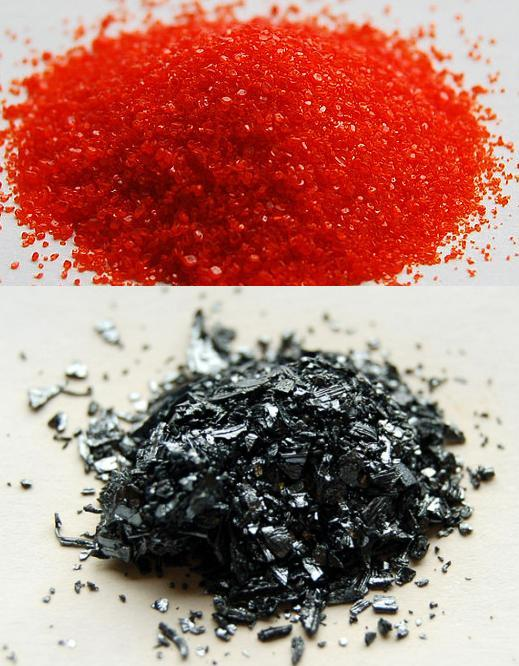
\includegraphics[width=.7\textwidth]{photos/iodine-KCr2O7-wikipedia.jpg}\par
\begin{caption}Kaliumdichromaat (bo) en jodium (onder)\end{caption}
\end{center}
}

\end{minipage}
}
\end{activity}

\begin{exercises}{Mengsels}
{Voltooi die volgende tabel: \par
%\nopagebreak
\begin{tabular}{|l|l|l|l|}\hline
\textbf{Stof} & \textbf{Nie-mengsel of} & \textbf{Heterogene} & \textbf{Homogene} \\ 
 & \textbf{mengsel} & \textbf{mengsel} & \textbf{mengsel} \\ \hline
kraanwater & & & \\ \hline
brons ( 'n allooi van koper en sink) & & & \\ \hline
beton & & & \\ \hline
aluminiumfolie & & & \\ \hline
Coca Cola & & & \\ \hline
seperige water & & & \\ \hline
swart tee & & & \\ \hline
suikerwater & & & \\ \hline
baba-melk formule & & & \\ \hline
\end{tabular}

\practiceinfo
\begin{tabular}[h]{cccccc}
 (1.) llm  &
\end{tabular} 
}
\end{exercises}


\section{Suiwer stowwe: Elemente en verbindings}
\nopagebreak
Enige stof wat nie 'n mengsel is nie, word 'n \textbf{suiwer stof} genoem. Suiwer stowwe sluit \textbf{elemente} en \textbf{verbindings} in. Dit is baie moeiliker om suiwer stowwe in hul dele af te breek, ingewikkelde chemiese metodes is nodig om dit te doen.\par

\mindsetvid{Classifying matter}{VPacc} 

Chromatografie is die proses van die skeiding van stowwe in hul individuele komponente. As 'n stof suiwer is, sal chromatografie slegs 'n enkel stof aan die einde van die proses oplewer. As 'n stof onsuiwer is sal verskeie stowwe aan die einde van die proses sien.\par

\begin{activity}{Voorgestelde praktiese aktiwiteit: Smartie chromatografie}{
Jy benodig:
\begin{itemize}[noitemsep]
\item filtreerpapier (of kladpapier)
\item 'n paar Smarties in verskillende kleure
\item water
\item an oogdrupper
\end{itemize}
\begin{minipage}{.5\textwidth}
Plaas 'n Smartie in die middel van 'n stukkie filtreerpapier. Drup versigtig 'n paar druppels water op die Smartie, totdat die Smartie goed nat is en daar 'n ring van water op die filtreerpapier vorm. Na 'n rukkie behoort jy 'n gekleurde ring op die papier rondom die Smartie waar te neem. Dit is omdat die voedselkleursel, wat gebruik was om die Smartie te kleur, in die water opgelos het en deur die papier weg van die Smartie af beweeg het.
\end{minipage}
\begin{minipage}{.5\textwidth}
\begin{center}
 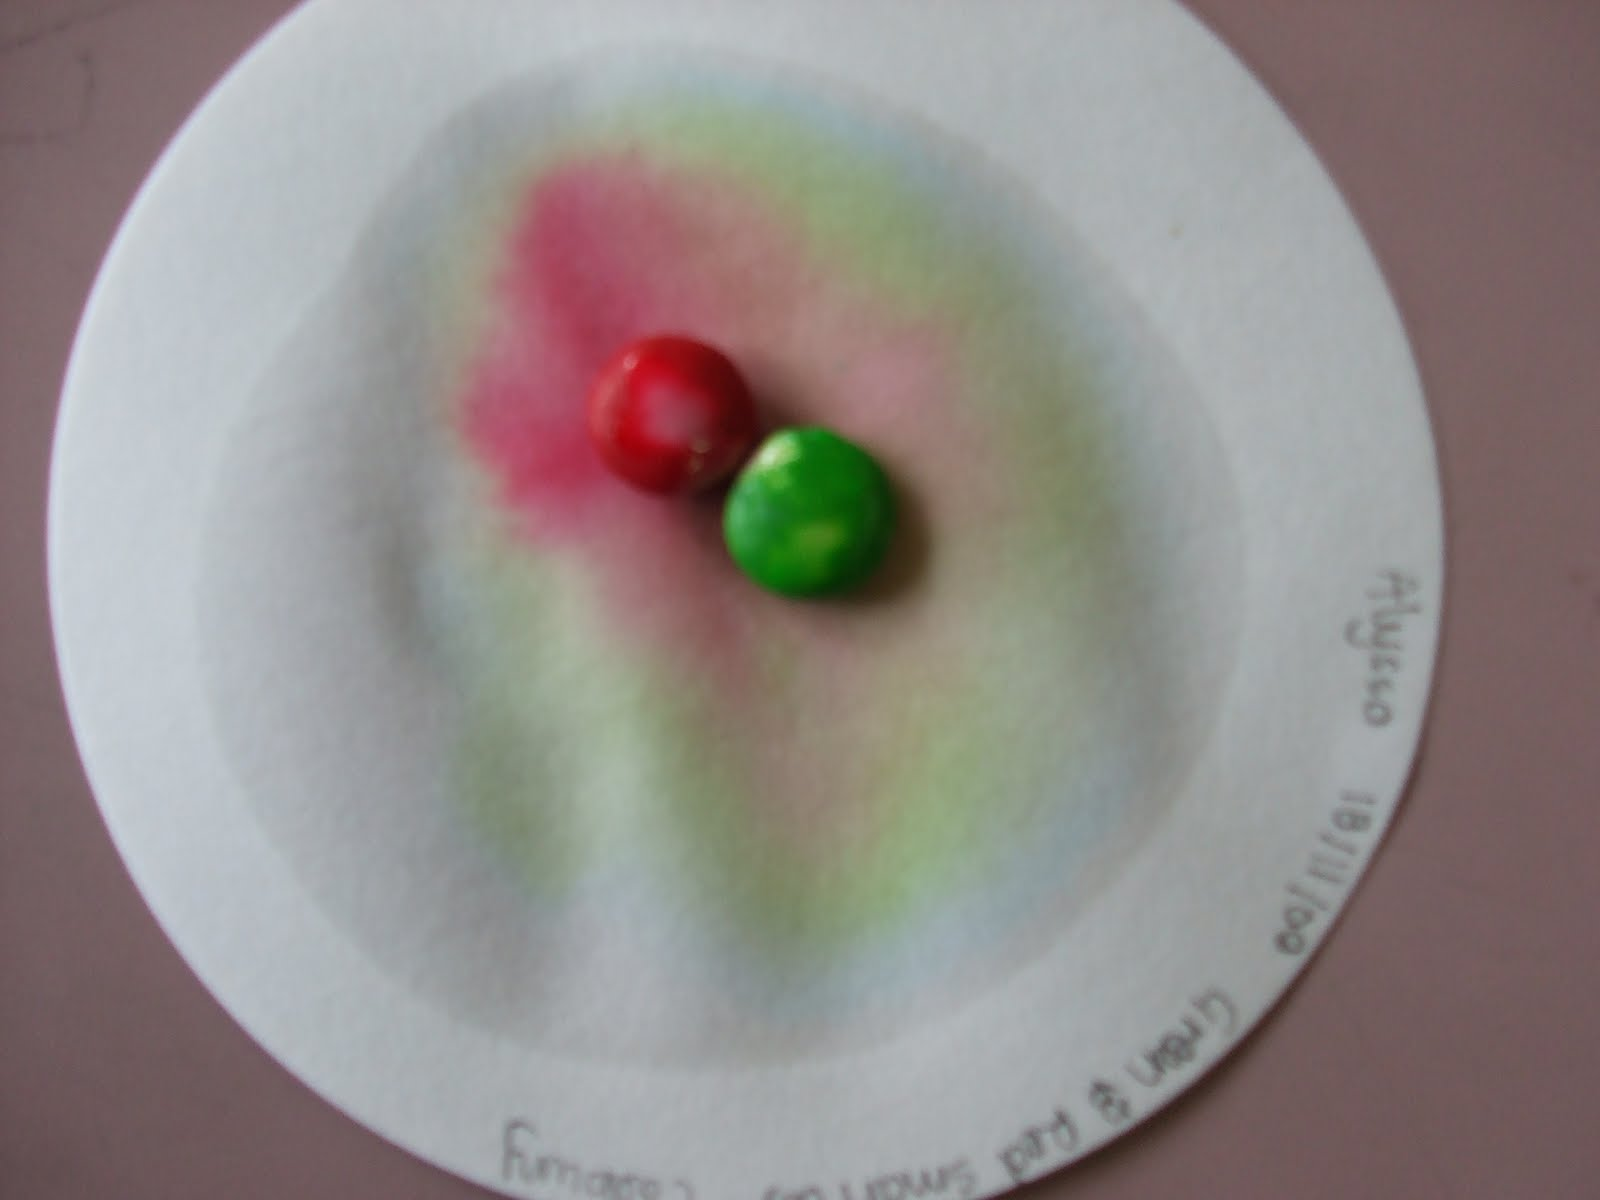
\includegraphics[width=.8\textwidth]{photos/smartie2.jpg}\par
\textit{Prent verskaf deur Neil Ravenscroft - UCT}
\end{center}
\end{minipage}
}
\end{activity}
\par 
	\par
      \label{m38708*uid25}
            \subsection*{Elemente}
            \nopagebreak
        \label{m38708*id63302} 'n \textbf{Element} is 'n chemiese stof wat nie verdeel of verander kan word in ander chemiese stowwe deur gewone chemiese metodes nie. Die kleinste eenheid van 'n element is die \textbf{atoom}.\par 
\label{m38708*fhsst!!!underscore!!!id193}
\Definition{   \label{id2406278} Element } 
{ \label{m38708*meaningfhsst!!!underscore!!!id193}
 'n Element is 'n stof wat nie in ander stowwe opgebreek kan word deur chemiese metodes nie.} 
        \label{m38708*id63334}Daar is amptelik 112 benoemde elemente waarvan omtrent 118 bekende elemente is. Meeste van hierdie elemente kom natuurlik voor, maar sommige is mensgemaak. Die elemente wat ons ken word in die \textbf{Periodieke Tabel van die Elemente} voorgestel. Elke element word tot 'n \textbf{chemiese simbool} afgekort. Tabel \ref{tab:elements} gee die eerste 20 elemente en 'n paar van die algemene oorgangsmetale.\par \label{m38708*eip-775}

\IFact{Onlangs is ooreengekom dat twee bykomende elemente tot die amptelike lys van benoemde elemente gevoeg word. Dit is elemente nommer 114 en 116. Die voorgestelde naam vir element 114 is flerovium en vir element 116 is dit moskovium. Dit bring die totale aantal amptelik benoemde elemente tot 114.}
\begin{table}[h!]
\label{tab:elements}
\begin{center}
\begin{tabular}{|l|l|l|l|}\hline
\textbf{Element naam} & \textbf{Element simbool} & \textbf{Element naam} & \textbf{Element simbool} \\ \hline
Waterstof & $\text{H}$ & Fosfor & $\text{P}$  \\ \hline
Helium & $\text{He}$ & Swawel & $\text{S}$ \\ \hline
Litium & $\text{Li}$ & Chloor & $\text{Cl}$ \\ \hline
Berillium & $\text{Be}$ & Argon & $\text{Ar}$ \\ \hline 
Boor & $\text{B}$ & Kalium & $\text{K}$ \\ \hline
Koolstof & $\text{C}$ & Kalsium & $\text{Ca}$ \\ \hline 
Stikstof & $\text{N}$ & Yster & $\text{Fe}$ \\ \hline
Suurstof & $\text{O}$ & Nikkel & $\text{Ni}$ \\ \hline 
Fluoor & $\text{F}$ & Koper & $\text{Cu}$ \\ \hline
Neon & $\text{Ne}$  & Sink & $\text{Zn}$ \\ \hline
Natrium & $\text{Na}$  & Silwer & $\text{Ag}$ \\ \hline
Magnesium & $\text{Mg}$  & Platinum & $\text{Pt}$ \\ \hline
Aluminium & $\text{Al}$ & Goud & $\text{Au}$ \\ \hline
Silicon & $\text{Si}$ & Kwik & $\text{Hg}$  \\ \hline
\end{tabular}
\end{center}
\caption{Lys van die eerste 20 elemente en 'n paar algemene oorgangsmetale}
\end{table}
\par 


      \label{m38708*uid26}
            \subsection*{Verbindings}
            \nopagebreak
        \label{m38708*id63363} 'n \textbf{Verbinding} is 'n chemiese stof wat gevorm word wanneer twee of meer verskillende elemente in 'n vaste verhouding verbind. Byvoorbeeld, Water ($\text{H}{}_{2}\text{O}$) is 'n verbinding wat bestaan uit twee waterstofatome vir elke een suurstofatoom. Natriumchloried ($\text{NaCl}$) is 'n verbinding wat bestaan uit een natriumatoom vir elke chlooratoom. 'n Belangrike eienskap van 'n verbinding is dat dit 'n \textbf{chemiese formule} het, wat die verhouding waarin die atome van elke element in die verbinding voorkom, beskryf.\par 
\label{m38708*fhsst!!!underscore!!!id201}
%\begin{definition}
%	  \begin{tabular*}{15 cm}{m{15 mm}m{}}
%	\hspace*{-50pt}  
\includegraphics[width=0.5in]{col11305.imgs/psflag2.png}   & 
\Definition{\label{id2406453} Verbinding } { \label{m38708*meaningfhsst!!!underscore!!!id201}
        'n Stof wat bestaan uit twee of meer verskillende elemente wat in 'n vaste verhouding saamgevoeg is.
         } 

\mindsetvid{Particles inside compounds}{VPacw} 

%       \end{tabular*}
%       \end{definition}
        \label{m38708*id63410} Figuur \ref{fig:classification:mixture and compound} kan jou help om die verskil tussen die terme \textbf{element}, \textbf{mengsel} en \textbf{verbinding} te verstaan. Yster ($\text{Fe}$) en swawel ($\text{S}$) is twee elemente. Wanneer hulle bymekaar gevoeg word, vorm hulle 'n \textbf{mengsel} van yster en swawel. Die yster en swawel, is nie aan mekaar verbind nie. Maar sodra die mengsel verhit word, word 'n nuwe \textbf{verbinding} gevorm, wat ystersulfied ($\text{FeS}$) genoem word.\par 
%     \setcounter{subfigure}{0}
 \begin{minipage}{.5\textwidth}
    \begin{center}
\scalebox{0.8}{
 \begin{pspicture}(0,-1)(11,4.7)
\SpecialCoor
%\psgrid[gridcolor=lightgray]
\def\fe{\pscircle[fillcolor=violet!20!gray!70!blue,fillstyle=solid](0,0){0.4}\rput(0,0){Fe}}
\def\s{\pscircle[fillcolor=yellow,fillstyle=solid](0,0){0.2}\rput(0,0){S}}
\def\fes{\fe \rput(0.6,0){\s}} 

\psframe(0,0)(4,4)
\rput(1.5,2){\s}
\rput{30}(3,1){\rput(1,1){\fe}\rput(1.5,2){\s}}
\rput{65}(1.55,1.33){\rput(1,1){\fe}\rput(1.5,2){\s}}
\rput{265}(2,3){\rput(-0.1,0.4){\fe}\rput(1.5,1.6){\s}}
\rput(2,0.6){\s}
\rput(1,1){\fe}
\rput(3,0.7){\fe}
\rput(2.4,2){\fe}
\rput(1.4,3.6){\s}
\psline(3.4,0.6)(4.2,0.6)
\uput[r](4.2,0.6){\parbox{1.5cm}{ 'n Atoom van die element yster ($\text{Fe}$)}}

\psline(3.5,3.5)(4.2,3.5)
\uput[r](4.2,3.5){\parbox{1.5cm}{ 'n Atoom van die element swawel ($\text{S}$)}}
% \rput(2,-0.5){\parbox{4cm}{A mixture of iron and sulphur}}

% \rput(7,0){
% \psframe(0,0)(4,4)
% \rput(1,2){\fes}
% \rput(1,1){\fes}
% \rput(3,0.7){\fes}
% \rput(1,3.5){\fes}
% \rput(3,3.2){\fes}
% \rput(2.4,2){\fes}
% \rput(2,-0.5){\parbox{4cm}{The compound iron sulphide (FeS)}}}

\end{pspicture}
}\\
\begin{caption} 'n Mengsel van yster en swawel\end{caption}
\label{fig:classification:mixture and compound}
    \end{center}
\end{minipage}
 \begin{minipage}{.5\textwidth}
  \begin{center}
   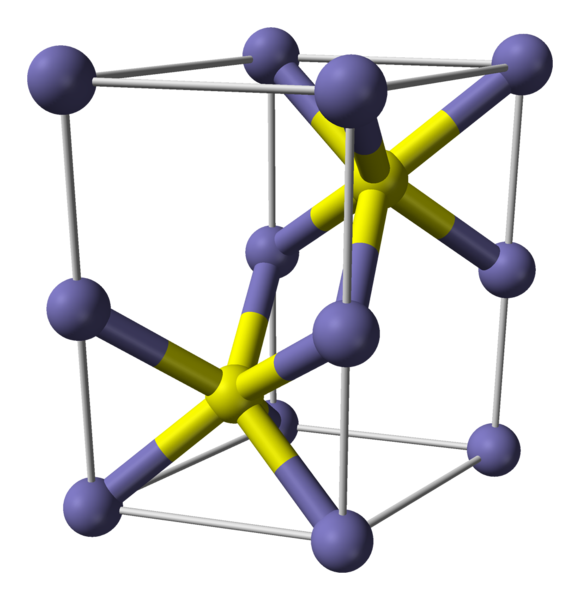
\includegraphics[width=0.4\textwidth]{photos/FeS_wikipedia.png}\\
\begin{caption} 'n Model van die ystersulfied kristal\end{caption}
  \end{center}

 \end{minipage}

\label{m38708*eip-487} Figuur \ref{fig:classification:mixture and compound} toon die submikroskopiese voorstelling van mengsels en verbindings. In 'n submikroskopiese voorstelling gebruik ons sirkels om verskillende elemente voor te stel. Om 'n verbinding te toon teken ons verskeie sirkels wat aanmekaar geheg is. Mengsels word eenvoudig as twee of meer afsonderlike elemente in dieselfde spasie aangedui. Die sirkels vir 'n mengsel is nie aanmekaar geheg nie.\par 
\label{m38708*id0124}Ons kan ook simbole gebruik om elemente, mengsels en verbindings voor te stel. Die simbole vir die elemente verskyn op die Periodieke Tabel. Verbindings word aangedui as twee of meer elementname wat reg langs mekaar geskryf word. Onderskrifte word gebruik om meer as een atoom van 'n spesifieke element aan te dui (bv. $\text{H}{}_{2}\text{O}$ of $\text{NH}_{3}$). Mengsels word geskryf as: 'n mengsel van die element (of verbinding) A en element (of verbinding) B. (bv. 'n mengsel van $\text{Fe}$ en $\text{S}$).\par 
\label{m38708*eip-524}
      \begin{wex}
{Mengsels en suiwer stowwe}
{Vir elk van die volgende stowwe stel of dit 'n suiwer stof of 'n mengsel is. As dit 'n mengsel is, is die mengsel homogeen of heterogeen? As dit 'n suiwer stof is, is dit 'n element of 'n verbinding?
\label{m38708*eip-id1167351497334}\begin{enumerate}[noitemsep, label=\textbf{\alph*}. ] 
   %         \leftskip=20pt\rightskip=\leftskip
\item Bloed (wat bestaan uit plasma en selle)
\item Argon
\item Silikondioksied ($\text{SiO}{}_{2}$)
\item Sand en klippe
\end{enumerate}
  }
%\vspace{5pt}
%\label{m38708*eip-62}\noindent\textbf{Solution to Exercise }
%\label{m38708*eip-id1167366034146}
{
\westep{Pas die definisies toe}
 'n Element word op die Periodieke Tabel gevind, so ons kyk na die Periodieke Tabel en vind dat slegs Argon daar verskyn. Vervolgens besluit ons watter is verbindings en watter is mengsels. Verbindings bestaan uit twee of meer elemente wat in 'n vaste verhouding verbind is. Sand en klippe is nie elemente nie, so ook nie bloed nie, maar silikon en suurstof is. Ten slotte besluit ons of die mengsel homogeen of heterogeen is. Aangesien ons nie die afsonderlike komponente van bloed kan sien nie is dit homogeen. Sand en klippe is heterogeen.
 %           \leftskip=20pt\rightskip=\leftskip
\westep{Skryf die antwoord neer}
\begin{enumerate}
[noitemsep, label=\textbf{\alph*}. ]
\item Bloed is 'n homogene mengsel.
\item Argon is 'n suiwer stof. Argon is 'n element.
\item Silikondioksied is 'n suiwer stof. Dit is 'n verbinding.
\item Sand en klippe vorm 'n heterogene mengsel.
\end{enumerate}}
    \end{wex}


  \label{m38708*eip-326}
\begin{activity}{Die gebruik van modelle om stowwe te verteenwoordig}{
\begin{minipage}{.5\textwidth}
Die volgende stowwe word gegee:
\label{m38708*eip-id1166921187210}
\begin{itemize}[noitemsep]
\item Lug (bestaande uit suurstof, stikstof, waterstof, waterdamp)
\item Waterstofgas ($\text{H}_{2}$)
\item Neongas
\item Stoom
\item Ammoniakgas ($\text{NH}_{3}$)
\end{itemize}
\end{minipage}
\begin{minipage}{.5\textwidth}
\begin{center}
 \includegraphics[width=.8\textwidth]{photos/models_classification.jpg}\par
\end{center}
\end{minipage}
\noindent
\begin{enumerate}[noitemsep, label=\textbf{\arabic*}.]
\item Gebruik gekleurde balle om modelle te bou vir elk van die stowwe wat gegee is.
\item Klassifiseer die stowwe as: elemente, verbindings, homogene mengsels, heterogene mengsel, suiwer stof, onsuiwer stof.
\item Teken submikroskopiese voorstelling vir elk van die bogenoemde voorbeelde.
\end{enumerate}

}
\end{activity}
%NTS add image here 
\par \label{m38708*secfhsst!!!underscore!!!id212}
            \begin{exercises}{Elemente, mengsels en verbindings}{
            \nopagebreak
            \label{m38708*id63472}
 \begin{enumerate}[noitemsep, label=\textbf{\arabic*}. ] 
            \label{m38708*uid28}
    \item Merk in die volgende tabel watter van die gegewe stowwe 'n \textsl{mengsel} of 'n \textsl{suiwer stof} is. As dit 'n mengsel is, sê ook of die mengsel homogeen of heterogeen is.
    % \textbf{m38708*id63499}\par
          \begin{table}[H]
    % \begin{table}[H]
    % \\ 'id2876023' '1'
        \begin{center}
      \label{m38708*id63499}
    \noindent
      \begin{tabular}{|l|l|l|}\hline
        \textbf{Stof} &
        \textbf{Mengsel of suiwer} &
        \textbf{Homogene of heterogene mengsel} \\ \hline
        bruis koeldrank & & \\ \hline
        staal & & \\ \hline
        suurstof & & \\ \hline
        ystervylsels & & \\ \hline
        rook & & \\ \hline
        kalksteen (${\text{CaCO}}_{3}$) & & \\ \hline
    \end{tabular}
      \end{center}
%    \begin{center}{\small\bfseries Table 1.1}\end{center}
%    \begin{caption}{\small\bfseries Table 1.1}\end{caption}
\end{table}
    \par
\label{m38708*uid29}\item In elk van die volgende gevalle, sê of die stof 'n element, 'n mengsel of 'n verbinding is.
\label{m38708*id63912}\begin{enumerate}[noitemsep, label=\textbf{\alph*}. ] 
            \label{m38708*uid30}\item $\text{Cu}$
\label{m38708*uid31}\item yster en swawel
\label{m38708*uid32}\item $\text{Al}$
\label{m38708*uid33}\item $\text{H}{}_{2}\text{SO}{}_{4}$
\label{m38708*uid34}\item $\text{SO}{}_{3}$\end{enumerate}
                \end{enumerate}

\practiceinfo
\begin{tabular}[h]{cccccc}
 (1.) lly  &  (2.) llV  & 
\end{tabular}
}
\end{exercises}
%NTS DIAGRAM is needed here and some more examples in the above exercises
            \section{Gee name en formules aan stowwe}
            \nopagebreak
      \label{m38708*eip-379}Dink na oor wat jy jou vriende noem. Sommige van jou vriende mag volle name (lang name) en 'n bynaam (kort naam) hê. Dit is die woorde wat ons gebruik om ander te vertel na wie of wat ons verwys. Hulle volle naam is soos die stowwe se naam; en hulle bynaam is soos stowwe se formules. Sonder hierdie name het jou vriende geen idee na wie van hulle jy verwys nie. Chemiese stowwe het name, net soos mense name het. Dit help wetenskaplikes om doeltreffend te kommunikeer. 
     \par \label{m38708*id64028}Dit is maklik om elemente en mengsels te beskryf. Ons gebruik eenvoudig die name wat ons op die Periodieke Tabel van elemente kry en gebruik woorde om mengsels te beskryf. Maar hoe word verbindings benoem? In die voorbeeld van ystersulfied wat vroeër gebruik is, is die saamgestelde naam 'n kombinasie van die name van die elemente, maar effens verander. \par 

\mindsetvid{why do chemical compounds form}{VPadm} 

      \label{m38708*id64033}Die volgende is 'n paar riglyne vir die benaming van verbindings:\par 


4. 'n Verbinding kan ione ( 'n ioon is 'n atoom wat elektrone verloor of bygekry het) bevat. Hierdie ione kan enkelvoudig (bestaan uit net een element) of meervoudig (bestaan uit verskeie elemente) wees. Sommige van die meer algemene ione en hul formules word in tabel 1.3 en tabel 1.4 gegee. Jy behoort al hierdie ione te ken.

      \label{m38708*id64037}\begin{enumerate}[noitemsep, label=\textbf{\arabic*}. ] 
            \label{m38708*uid35}\item Die verbinding se naam sal altyd die \textbf{name van die elemente} wat deel daarvan vorm insluit.
\label{m38708*id64059}\begin{itemize}[noitemsep]
            \label{m38708*uid36}\item 'n Verbinding van \textbf{yster} ($\text{Fe}$) en \textsl{swawel} ($\text{S}$) is \textbf{yster}\textsl{sulf}ied ($\text{FeS}$)
\label{m38708*uid37}\item 'n Verbinding van \textbf{kalium} ($\text{K}$) en \textsl{broom} ($\text{Br}$) is \textbf{kalium}\textsl{brom}ied ($\text{KBr}$)
\label{m38708*uid38}\item 'n Verbinding van \textbf{natrium} ($\text{Na}$) and \textsl{chloor} ($\text{Cl}$) is \textbf{natrium}\textsl{chlor}ied ($\text{NaCl}$)
\end{itemize}
        \label{m38708*uid39}\item In 'n verbinding, word die element aan die linkerkant van die Periodieke Tabel \textsl{eerste} gebruik by die benoeming van die verbinding. In die voorbeeld van $\text{NaCl}$, is natrium 'n groep 1 element op die linkerkant van die tabel, terwyl chloor in Groep 7 is aan die regterkant van die tabel. Natrium kom dus eerste in die verbinding se naam voor. Dieselfde geld vir $\text{FeS}$ en $\text{KBr}$.
\label{m38708*uid40}\item Die \textbf{simbole} van die elemente kan gebruik word om verbindings voor te stel, bv. $\text{FeS}$, $\text{NaCl}$, $\text{KBr}$ en $\text{H}{}_{2}\text{O}$. Dit word die chemiese formules genoem. In die eerste drie voorbeelde, is die verhouding van die elemente in elke verbinding 1:1. Dus is daar een atoom yster vir elke swawel atoom in die verbinding. In die laaste voorbeeld ($\text{H}{}_{2}\text{O}$) is daar twee atome waterstof vir elke atoom suurstof in die verbinding.
\item 'n Verbinding kan \textbf{ione} ( 'n ioon is 'n atoom wat elektrone verloor of bygekry het) bevat. Hierdie ione kan enkelvoudig (bestaan uit net een element) of meervoudig (bestaan uit verskeie elemente) wees. Sommige van die meer algemene ione en hul formules word in tabel \ref{tab:cations} en tabel \ref{tab:anions} gegee. Jy behoort al hierdie ione te ken.

    % \textbf{m38708*id64235}\par
    %      \begin{table}[H]
    % \begin{table}[H]
    % \\ 'id2876536' '1'

\begin{table}[H]
\begin{center}
\label{tab:cations}
\begin{tabular}{|l|c|l|c|l|c|l|c|} \hline
\textbf{Ioonverbinding} & \textbf{Formule} & \textbf{Ioonverbinding} & \textbf{Formule} & \textbf{Ioonverbinding} & \textbf{Formule}  \\ \hline
Waterstof       & $\text{H}^{+}$   & Litium          & $\text{Li}^{+}$     & Natrium          & $\text{Na}^{+}$  \\ \hline
Kalium          & $\text{K}^{+}$   & Silwer          & $\text{Ag}^{+}$     & Kwikk (I)        & $\text{Hg}^{+}$  \\ \hline
Koper (I)       & $\text{Cu}^{+}$  & Ammonium        & $\text{NH}_{4}^{+}$ & Berillium        & $\text{Be}^{2+}$ \\ \hline
Magnesium       & $\text{Mg}^{2+}$ & Kalsium         & $\text{Ca}^{2+}$    & Barium           & $\text{Ba}^{2+}$ \\ \hline
Tin (II)        & $\text{Sn}^{2+}$ & Lood (II)       & $\text{Pb}^{2+}$    & Chroom (II)      & $\text{Cr}^{2+}$ \\ \hline
Mangaan (II)    & $\text{Mn}^{2+}$ & Yster (II)      & $\text{Fe}^{2+}$    & Kobalt (II)      & $\text{Co}^{2+}$ \\ \hline
Nikkel          & $\text{Ni}^{2+}$ & Koper (II)      & $\text{Cu}^{2+}$    & Sink             & $\text{Zn}^{2+}$ \\ \hline
Aluminium       & $\text{Al}^{3+}$ & Chroom (III)    & $\text{Cr}^{3+}$    & Yster (III)      & $\text{Fe}^{3+}$ \\ \hline
Kobalt (III)    & $\text{Co}^{3+}$ & Chroom (VI)     & $\text{Cr}^{6+}$    & Mangaan (VII)    & $\text{Mn}^{7+}$ \\ \hline

\end{tabular}

 \end{center}
\caption{Tabel van katione}
\label{tab:cations}
\end{table}

\begin{table}[H]
\begin{center}
\label{tab:anions}
\begin{tabular}{|l|c|l|c|l|c|l|c|} \hline
\textbf{Ioonverbinding} & \textbf{Formule}            & \textbf{Ioonverbinding} & \textbf{Formule} \\ \hline
Fluoried                & $\text{F}^{-}$             & Oxied               & $\text{O}^{2-}$ \\ \hline
Chloried                & $\text{Cl}^{-}$            & Peroksied           & $\text{O}_{2}^{2-}$ \\ \hline
Bromied                 & $\text{Br}^{-}$            & Karbonaat           & $\text{CO}_{3}^{2-}$ \\ \hline
Jodied                  & $\text{I}^{-}$             & Sulfied             & $\text{S}^{2-}$ \\ \hline
Hidroksied              & $\text{OH}^{-}$            & Sulfiet             & $\text{SO}_{3}^{2-}$ \\ \hline
Nitriet                 & $\text{NO}_{2}^{-}$        & Sulfaat             & $\text{SO}_{4}^{2-}$ \\ \hline
Nitraat                 & $\text{NO}_{3}^{-}$        & Thiosulfaat         & $\text{S}_{2}{\text{O}}_{3}^{2-}$ \\ \hline
Waterstofkarbonaat      & $\text{HCO}_{3}^{-}$       & Chromaat            & $\text{CrO}_{4}^{2-}$ \\ \hline
Waterstofsulfiet        & $\text{HSO}_{3}^{-}$       & Dichromaat          & $\text{Cr}_{2}{\text{O}}_{7}^{2-}$ \\ \hline
Waterstofsulfaat        & $\text{HSO}_{4}^{-}$       & Manganaat           & $\text{MnO}_{4}^{2-}$ \\ \hline
Diwaterstoffosfaat      & $\text{H}_{2}{\text{PO}}_{4}^{-}$ & Oksalaat     & $\text{(COO)}_{2}^{2-}/{\text{C}}_{2}{\text{O}}_{4}^{2-}$ \\ \hline
Hipochloriet            & $\text{ClO}^{-}$           & Waterstoffosfaat    & $\text{HPO}_{4}^{2-}$ \\ \hline
Chloraat                & $\text{ClO}_{3}^{-}$       & Nitried             & $\text{N}^{3-}$ \\ \hline
Permanganaat            & $\text{MnO}_{4}^{-}$       & Fosfaat             & $\text{PO}_{4}^{3-}$ \\ \hline
Asetaat Etanoaat        & $\text{CH}_{3}{\text{COO}}^{-}$   & Fosfied      & $\text{P}^{3-}$ \\ \hline
\end{tabular}

 \end{center}
\caption{Tabel van anione}
\label{tab:anions}
\end{table}

    \par
  \label{m38708*uid42}\item Wanneer daar slegs twee elemente in die verbinding is, kry die verbinding dikwels die \textbf{agtervoegsel} (op die end) \textbf{–ied}. Jy sou dit reeds opgelet het in sommige van die voorbeelde wat ons tot dusver gebruik het. Vir saamgestelde ione, wanneer 'n nie-metaal met suurstof verbind om 'n negatiewe ioon (anioon) te vorm wat dan weer met 'n positiewe ioon (katioon) soos waterstof of 'n metaal verbind, is die agtervoegsel van die naam \textbf{–aat} of \textbf{–iet}. By voorbeeld, $\text{NO}_{3}^{-}$ is 'n negatiewe ioon, wat kan verbind met 'n katioon soos waterstof ($\text{HNO}{}_{3}$) of 'n metaal soos kalium ($\text{KNO}{}_{3}$). Die $\text{NO}_{3}^{-}$ anioon het die naam nitr\textbf{aat}. $\text{SO}_{3}^{2-}$ in 'n formule is sulf\textbf{iet}, bv. natriumsulf\textbf{iet} ($\text{Na}{}_{2}\text{SO}{}_{3}$). $\text{SO}_{4}^{2-}$ is sulf\textbf{aat} en $\text{PO}_{4}^{3-}$ is fosf\textbf{aat}.
\label{m38708*uid43}\item \textbf{Voorvoegsels} kan gebruik word om die verhouding van die elemente in die verbinding te beskryf. Dit word vir nie-metale gebruik. Vir metale, voeg ons 'n romeinse syfer (I, II, III, IV) in hakies na die metaalioon om die verhouding aan te dui. Jy behoort die volgende voorvoegsels te ken: "mono" (een), "di" (twee) en 'tri " (drie).
\label{m38708*id64977}\begin{itemize}[noitemsep]
            \label{m38708*uid44}\item $\text{CO}$ (koolstof\textbf{mon}oksied) - Daar is een suurstof atoom suurstof vir elke een koolstof atoom
\label{m38708*uid45}\item $\text{NO}{}_{2}$ (stikstof\textbf{di}oksied) - Daar is twee suurstof atome vir elke een stikstof atoom
\label{m38708*uid46}\item $\text{SO}{}_{3}$ (swawel \textbf{tri}oksied) - Daar is drie suurstof atome vir elke een swawel atoom
\end{itemize}
        \end{enumerate}
\label{m38708*id537402}Bogenoemde riglyne help ons ook om vanaf die naam van die verbinding die formule van 'n verbinding uit te werk.\par 
\label{m38708*eip-178}Wanneer die formule van 'n verbinding uitgewerk word, werk ons terugwaarts. By voorbeeld, as jy gevra word om die formule van kaliumchloried te gee, begin deur daarop te let dat ons kalium en chloried het. Skryf vervolgens die formule neer vir elk van hierdie ione. Kalium is ${\text{K}}^{+}$ en chloried is ${\text{Cl}}^{-}$. Die finale stap is om te let op die lading op elke ioon en te kyk hoe die ladings kombineer. Aangesien beide kalium en chloor 'n lading van 1 het, verbind hulle in 'n 1:1 verhouding. Die formule is $\text{KCl}$.\par \label{m38708*notfhsst!!!underscore!!!id252}
%\begin{tabular}{cc}
%	   \hspace*{-50pt}\raisebox{-8 mm}{ 
\includegraphics[width=0.5in]{col11305.imgs/pstip2.png}  }& 
%	\begin{minipage}{0.85\textwidth}
%	\begin{note}
\Tip{Wanneer getalle as onderskrifte in verbindings (dit wil sê hulle word onder en aan die regterkant van die element se simbool geskryf) geskryf word, sê dit vir ons hoeveel atome van daardie element daar is in verhouding tot die ander elemente in die verbinding. Byvoorbeeld in stikstofdioksied (${\text{NO}}_{2}$) is daar twee suurstof atome vir elke een stikstof atoom. Later, wanneer ons begin kyk na chemiese vergelykings, sal jy agterkom dat daar somtyds nommers \textbf{voor} die naam van die verbindings is. So beteken $2\text{H}{}_{2}\text{O}$, byvoorbeeld, dat daar twee molekules water is en dat daar in elke molekule twee waterstofatome vir elke een suurstof atoom is.\par}  
%	\end{note}
%	\end{minipage}
%	\end{tabular}
	\par
\label{m38708*eip-163}Ons kan hierdie reëls gebruik om ons te help met die naam van beide ioniese verbindings en kovalente verbindings. Wetenskaplikes gee egter dikwels ander name vir kovalente verbindings om die naam te vereenvoudig (of omdat die molekuul benoem was lank voordat die formule ontdek is). Byvoorbeeld, as ons 2 waterstofatome en 1 suurstofatoom het, sal volgens bogenoemde benamingsreëls die naam van die stof diwaterstofmonoksied wees. Maar hierdie verbinding is beter bekend as water!  \par \label{m38708*eip-254} 

\begin{wex}{Skryf die chemiese formules 1}
{Wat is die formule vir natriumfluoried? }
{\westep {Noem die ione wat betrokke is:}
Ons het die natriumioon ($\text{Na}^{+}$) en die fluoriedioon ($\text{Fl}^{-}$). (Jy kan dit op die tabelle van anione en katione naslaan.)
\westep{Skryf die ladings van die ione neer:}
Natrium het 'n lading van $+1$ en fluoor het 'n lading van $-1$.
\westep{Vind die regte kombinasie:}
Vir elke plus moet daar 'n minus wees. Dus benodig die $+1$ natriumioon een $-1$ fluoriedioon sodat die lading gebalanseer is. Natrium en fluor verbind in 'n 1:1 verhouding.
\westep{Skryf die formule neer:}
$\text{NaFl}$
}
\end{wex}
      \begin{wex}{Skryf die chemiese formules 2}
{Wat is die formule vir magnesiumchloried? }
{\westep {Noem die ione wat betrokke is:}
Ons het die magnesiumioon ($\text{Mg}^{2+}$) en die chloriedioon ($\text{Cl}^{-}$).
\westep{Skryf die ladings van die ione neer:}
Magnesium het 'n lading van $+2$ en chloor het 'n lading van $-1$.
\westep{Vind die regte kombinasie:}
Vir elke plus moet daar 'n minus wees. Dus benodig die $+2$ magnesiumioon twee $-1$ chloriedione sodat die lading gebalanseer is. Magnesium en chloor verbind in 'n 1:2 verhouding. Daar is 'n eenvoudige manier om hierdie verhouding te bepaal:
\begin{figure}[H] % horizontal\label{m38708*uid27}
    \begin{center}
 \begin{pspicture}(0,0)(2,2)
\SpecialCoor
\psline[linewidth=0.04]{->}(0,1)(1,0)
\uput[r](-1.2,1){\large{$\text{Mg}^{2+}$}}
\psline[linewidth=0.04]{->}(0,0)(1,1)
\uput[r](-1,0){\large{$\text{Cl}^{-}$}}
\uput[r](1,1){\large{$2$}}
\uput[r](1,0){\large{$1$}}

\end{pspicture}
\end{center}
\end{figure}
Teken 'n kruis soos bo aangedui en kyk dan hoe $\text{Mg} \rightarrow 1$ en $\text{Cl} \rightarrow 2$. 
\westep{Skryf die formule neer:}
$\text{MgCl}{}_{2}$
}
\end{wex} 

    
    \noindent

      \noindent
      \begin{wex}{Skryf die chemiese formules 3}
{Wat is die formule vir magnesiumoksied? }
{\westep {Noem die ione wat betrokke is:}
Ons het die magnesiumioon ($\text{Mg}^{2+}$) en die chloriedioon ($\text{O}^{2-}$).
\westep{Vind die regte kombinasie:}
$\text{Mg}^{2+} : 2$ \newline
$\text{O}^{2-} : 2$ \newline
As jy die kruismetode gebruik, sal jy 'n verhouding van $2:2$ kry. Hierdie verhouding moet altyd in sy eenvoudigste vorm gegee word, m.a.w. $1:1$.
\westep{Skryf die formule neer:}
$\text{MgO}$
}
\end{wex}

      \begin{wex}{Skryf die chemiese formules 4}
{Wat is die formule vir koper(II)nitraat? }
{\westep {Noem die ione wat betrokke is:}
$\text{Cu}^{2+}$ (die vraag s\^e koper(II), nie koper(I) nie) \newline
$\text{NO}_{3}^{-}$
\westep{Vind die regte kombinasie:}
	\begin{figure}[H] % horizontal\label{m38708*uid27}
    \begin{center}
 \begin{pspicture}(0,0)(2,2)
\SpecialCoor
\psline[linewidth=0.04]{->}(0,1)(1,0)
\uput[r](-1,1){\large{$\text{Cu}^{2+}$}}
\psline[linewidth=0.04]{->}(0,0)(1,1)
\uput[r](-1.2,0){\large{$\text{NO}_{3}^{-}$}}
\uput[r](1,1){\large{$2$}}
\uput[r](1,0){\large{$1$}}

\end{pspicture}
\end{center}
\end{figure}
\westep{Skryf die formule neer:}
${\text{Cu}}({\text{NO}}_{3})_{2}$
}
\end{wex}

\Tip{Let op hoe ons in die laaste voorbeeld $\text{NO}_{3}^{-}$ binne die hakies geskryf het. Ons doen dit om aan te dui dat $\text{NO}_{3}^{-}$ 'n saamgestelde ioon is en dat daar twee van hierdie ione aan een koperioon verbind is.}

\begin{activity}{Die ioon-maat-soek speletjie}
Jou onderwyser sal aan elkeen van julle 'n ander ioon toeken (geskryf op 'n kaartjie). Plak dit op jou. Jy sal ook kaarte kry met die syfers 1 - 5 op. Loop nou in die klas rond en soek  'n maat, hou in gedagte watter ioon by jou kan pas en in watter verhouding. Sodra jy 'n maat gevind het, gee  'n aanduiding van die verhouding van elke ioon deur die genommerde kaarte te gebruik. Kontroleer jou resultate met jou klasmaats of jou onderwyser.
\end{activity}

  \label{m38708*secfhsst!!!underscore!!!id255}
            \begin{exercises}{Name van Verbindings}
{            \nopagebreak \noindent
      \label{m38708*id65118}\begin{enumerate}[noitemsep, label=\textbf{\arabic*}. ] 
            \label{m38708*uid47}\item Die formule vir kalsiumkarbonaat $\text{CaCO}{}_{3}$.
\label{m38708*id65148}\begin{enumerate}[noitemsep, label=\textbf{\alph*}. ] 
            \label{m38708*uid48}\item Is kalsiumkarbonaat 'n element of 'n verbinding? Gee 'n rede vir jou antwoord.
\label{m38708*uid49}\item Wat is die verhouding van $\text{Ca}:\text{C}:\text{O}$ atome in die formule?
\end{enumerate}
\label{m38708*uid50}\item Gee die naam van elk van die volgende stowwe.
\label{m38708*id65189}\begin{enumerate}[noitemsep, label=\textbf{\alph*}. ] 
            \label{m38708*uid51}\item $\text{KBr}$
\label{m38708*uid52}\item $\text{HCl}$
\label{m38708*uid53}\item ${\text{KMnO}}_{4}$\label{m38708*uid54}\item ${\text{NO}}_{2}$\label{m38708*uid55}\item ${\text{NH}}_{4}\text{OH}$
\label{m38708*uid56}\item ${\text{Na}}_{2}{\text{SO}}_{4}$
\item ${\text{Fe}}({\text{NO}}_{3})_3$
\item ${\text{Pb}}{\text{SO}}_{3}$
\item ${\text{Cu}}({\text{HCO}}_{3})_2$
\end{enumerate}
\label{m38708*uid57}\item Gee die chemiese formule vir elk van die volgende verbindings.
\label{m38708*id65338}\begin{enumerate}[noitemsep, label=\textbf{\alph*}. ] 
            \label{m38708*uid58}\item Kaliumnitraat
\label{m38708*uid59}\item Natriumoksied
\label{m38708*uid60}\item Bariumsulfaat
\label{m38708*uid61}\item Aluminiumchloried
\label{m38708*uid62}\item Magnesiumfosfaat
\item Tin(II)bromied
\item Mangaan(II)fosfied
\end{enumerate}
\end{enumerate}

\practiceinfo
\begin{tabular}[h]{cccccc}
 (1.) llp  &  (2.) lld  &  (3.) llv   & & 
\end{tabular}
}
\end{exercises}
%The above exercise needs more examples and some diagrams! Possibly also lost a curly brace
            \section{Metale, Metallo\"iede and Nie-metale}
%ADD a simple periodic table here to show this
            \nopagebreak
      \label{m38708*id65693}Die elemente in die Periodieke Tabel kan ook op grond van hulle eienskappe verdeel word as \textbf{metale}, \textbf{metallo\"iede} of \textbf{nie-metale}. Die sigsaglyn (zigzag) skei al die metaalelemente van die nie-metale. Metale word aan die linkerkant van die lyn gevind, en die nie-metale is aan die regterkant. Langs die lyn vind jy die metalloïde. Jy behoort daarop te let dat daar meer metale as nie-metale is. Metale, metalloïede en nie-metale het almal hul eie spesifieke eienskappe.\par 

\mindsetvid{classifying matter}{VPaec} 

\begin{figure}[h]

\begin{center}
\scalebox{0.7}{
\begin{pspicture}(-2,-2)(20,10)
%\psgrid[gridcolor=gray]
\psset{unit=1}
\pspolygon[fillstyle=solid,fillcolor=teal!20!white](0,3)(0,4)(1,4)(1,3)(0,3)
\pspolygon[fillstyle=solid,fillcolor=lightgray](0,-1)(0,3)(2,3)(2,1)(12,1)(12,2)(13,2)(13,0)(14,0)(14,-1)(0,-1)
\pspolygon[fillstyle=solid,fillcolor=cyan!50!white](12,2)(12,3)(13,3)(13,2)(12,2)
\pspolygon[fillstyle=solid,fillcolor=cyan!50!white](13,0)(13,2)(14,2)(14,1)(15,1)(15,0)(16,0)(16,-1)(14,-1)(14,0)(13,0)
\pspolygon[fillstyle=solid,fillcolor=teal!20!white](14,2)(13,2)(13,3)(17,3)(17,4)(18,4)(18,-1)(16,-1)(16,0)(15,0)(15,1)(14,1)(14,2)
\uput[l](4,0){\Huge{Metals}}
\uput[l](15.1,0.5){\LARGE{Metalloids}}
\uput[l](13.1,2.5){\Large{Metalloids}}
\uput[l](17.6,1.8){\Huge{Non-metals}}
\uput[l](0.9,3.5){\Huge{H}}
\end{pspicture}
}
\end{center}
\caption{ 'n Vereenvoudigde diagram wat  'n gedeelte van die Periodieke Tabel aantoon.}
\label{fig:periodic}
\end{figure} 
      \label{m38708*uid76}
            \subsection*{Metale}
            \nopagebreak
\begin{minipage}{.5\textwidth}
        \label{m38708*id65726}Voorbeelde van metale sluit in koper ($\text{Cu}$), sink ($\text{Zn}$), goud ($\text{Au}$), silwer ($\text{Ag}$), tin ($\text{Sn}$) en lood ($\text{Pb}$). Die volgende is sommige van die eienskappe van metale:\par 
\end{minipage}
\begin{minipage}{.5\textwidth}
\begin{center}
 \includegraphics[width=.2\textwidth]{photos/copperwire.jpg}
\end{center}
\end{minipage}

        \label{m38708*id65732}\begin{itemize}[noitemsep]
            \label{m38708*uid77}\item \textsl{Termiese geleiers} \\
       Metale is goeie geleiers van hitte en word dus gebruik in kombuis gereedskap soos potte en panne.
\label{m38708*uid78}\item \textsl{Elektriese geleiers} \\
       Metale is goeie geleiers van elektrisiteit en word dus gebruik in elektriese geleidingsdrade.
\label{m38708*uid79}\item \textsl{Blink metaalglans} \\
       Metale het 'n kenmerkende blink voorkoms en word dikwels gebruik om juweliersware te maak.
\label{m38708*uid80}\item \textsl{Smeebaar en pletbaar} \\
       Dit beteken dat hulle kan in  'n vorm gebuig word sonder om te breek (smeebaar) en kan uitgerek word in dun drade
      (rekbaar) soos koper.
\label{m38708*uid81}\item \textsl{Smeltpunt} \\
       Metale het gewoonlik 'n hoë smeltpunt en kan dus gebruik word om kookpotte te maak 
      en ander toerusting wat baie warm kan word, sonder om te beskadig.
\label{m38708*uid82}\item \textsl{Digtheid} \\
       Metale het 'n hoë digtheid.
\item \textsl{Magnetiese eienskappe} \\ 
       Slegs drie hoofmetale (yster, kobalt en nikkel) is magneties, die ander is nie-magneties.
\end{itemize}
         \label{m38708*id65852}Dit hoort duidelik te wees hoe die eienskappe van metale hul baie nuttig maak vir sekere doeleindes.\par 
\label{m38708*secfhsst!!!underscore!!!id320} 
            \begin{activity}{Groep Werk : 1. Kyk na metale}{
            \nopagebreak
\begin{minipage}{0.5\textwidth}
        \label{m38708*id65869}\begin{enumerate}[noitemsep, label=\textbf{\arabic*}. ]
            \label{m38708*uid83}\item Versamel 'n paar metaal-items by jou huis of skool. Hieronder is  'n paar voorbeelde:
\label{m38708*id65885}\begin{itemize}[noitemsep]
            \label{m38708*uid84}\item haarknippies
\label{m38708*uid85}\item haakspelde
\label{m38708*uid86}\item kookpotte
\label{m38708*uid87}\item juwele
\label{m38708*uid88}\item sk\^er
\label{m38708*uid89}\item eetgerei (messe, vurke, lepels)
\end{itemize}
        \label{m38708*uid90}\item In groepe van 3-4, voeg jou versameling metaal voorwerpe by die ander.
\label{m38708*uid91}\item Wat is die funksie van elk van hierdie voorwerpe?
\label{m38708*uid92}\item Bespreek waarom jy dink metaal is gebruik om elk van die voorwerpe te maak. Oorweeg die eienskappe van metale wanneer jy hierdie vraag beantwoord. 
\end{enumerate}
\end{minipage}
\begin{minipage}{.5\textwidth}
\begin{center}
 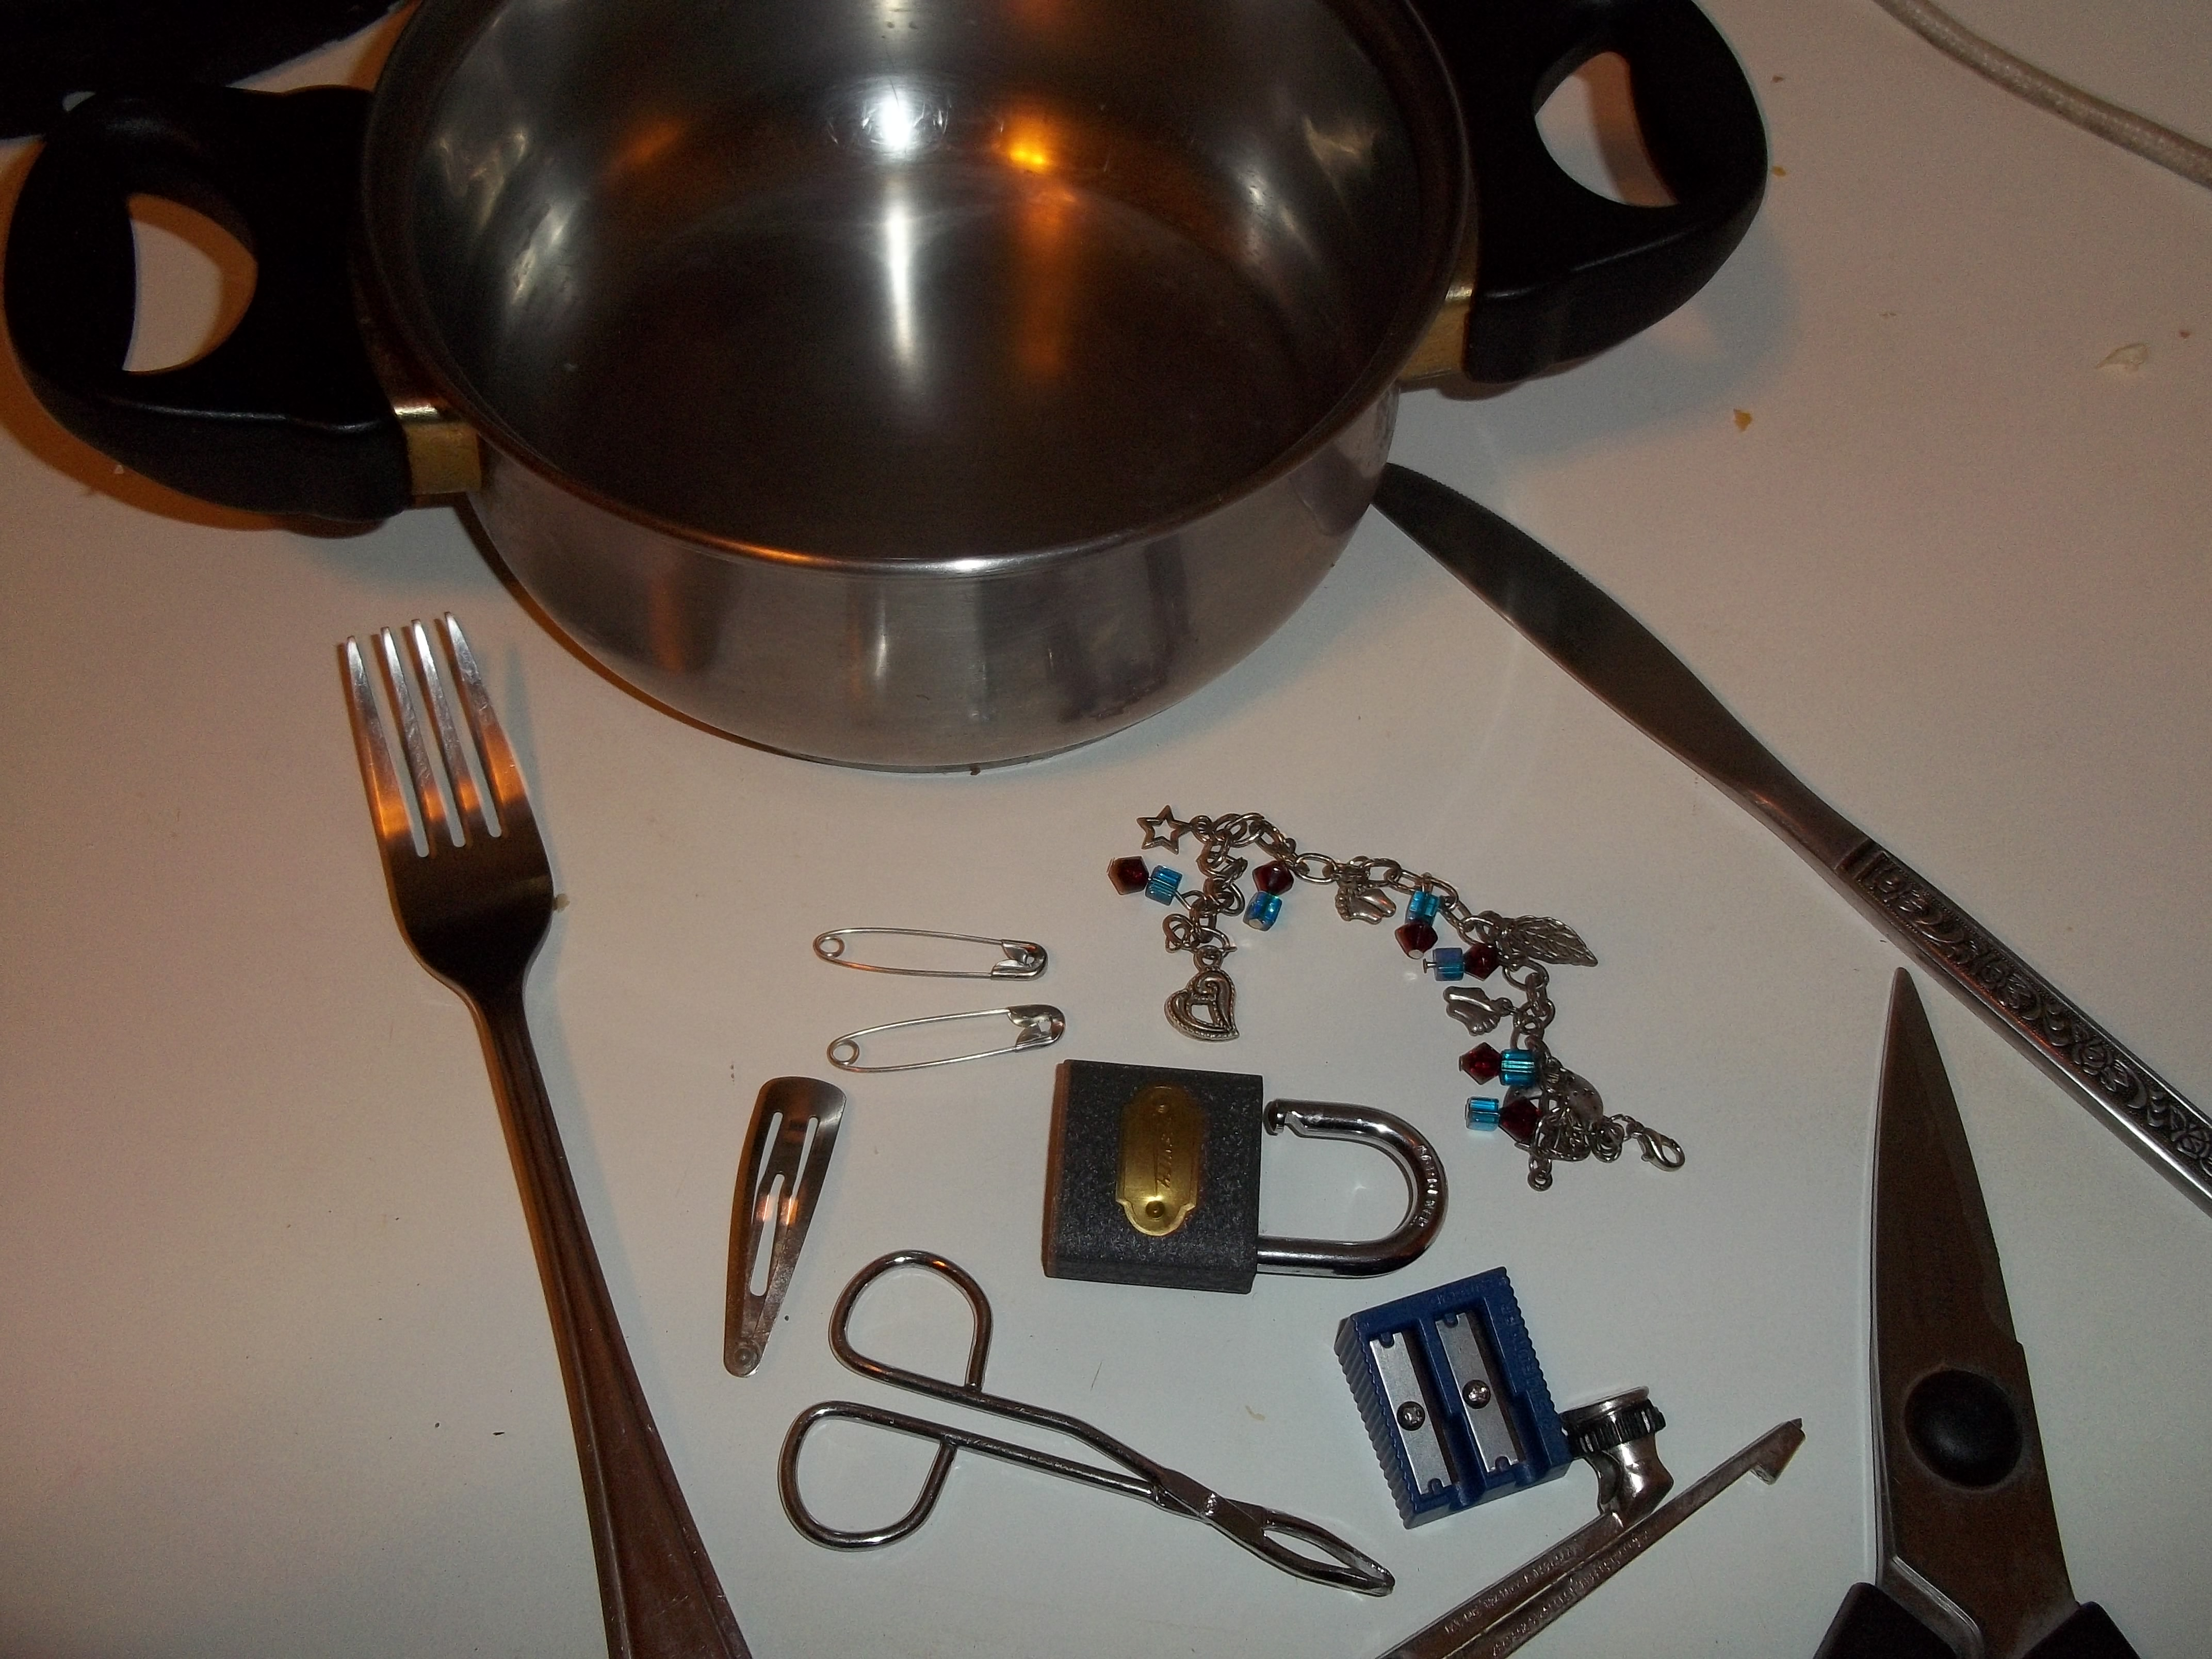
\includegraphics[width=.8\textwidth]{photos/metal_objects.jpg}\par
\end{center}
\end{minipage}
}
\end{activity}
      \label{m38708*uid93}
            \subsection*{Nie-metale}
            \nopagebreak
\begin{minipage}{.5\textwidth}
        \label{m38708*id66021}In teenstelling met metale, is nie-metale swak termiese geleiers, goeie elektriese isoleerders (wat beteken dat hulle \textsl{nie} elektrisiteit gelei nie) en nie pletbaar of smeebaar nie. Die nie-metale sluit elemente soos swawel ($\text{S}$), fosfor ($\text{P}$), stikstof ($\text{N}$) en suurstof ($\text{O}$) in.\par 
\end{minipage}
\begin{minipage}{.5\textwidth}
\begin{center}
 \includegraphics[width=.4\textwidth]{photos/sulphurby-nickstone333.jpg}\par
\textit{Prent verskaf deur nickstone333 op Flickr.com}
\end{center}
\end{minipage}
      \label{m38708*uid94}
            \subsection*{Metallo\"iede}
            \nopagebreak
\begin{minipage}{.5\textwidth}
        \label{m38708*id66042}Metalloïede of semi-metale, het meestal nie-metaaleienskappe. Een van hulle onderskeidende eienskappe is dat hulle geleidingsvermoë toeneem as hul temperatuur verhoog. Dit is die teenoorgestelde van wat gebeur in metale.  Di\'e eienskap is bekend as halfgeleiding en die stof word  'n halfgeleier genoem. Halfgeleiers is belangrik in elektronika, soos rekenaars en selfone. Die metallo\"iede sluit elemente soos silikon ($\text{Si}$) en germanium ($\text{Ge}$) in.\par 
\end{minipage}
\begin{minipage}{.5\textwidth}
\begin{center}
 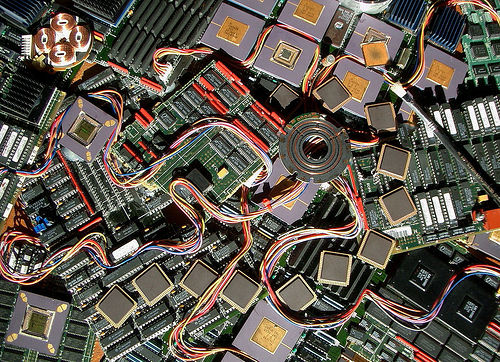
\includegraphics[width=.6\textwidth]{photos/siliconby-jurveston.jpg}\par
\textit{Prent verskaf deur jurveston op Flickr.com}
\end{center}
\end{minipage}
\par 
      \noindent
   %   \hspace*{-30pt}
\includegraphics[width=0.5in]{col11305.imgs/pspencil2.png}   \raisebox{25mm}{   
   %   \begin{mdframed}[linewidth=4, leftmargin=40, rightmargin=40]  
%       \begin{wex}{Metals, metalloids and non-metals 1}{\label{m38708*eip-77}
%   \label{m38708*eip-252}
% For each of the following substances state whether they are metals, metalloids or non-metals, using their position on the periodic table.
% \label{m38708*eip-id1170734629720}
% \begin{enumerate}[noitemsep, label=\textbf{\alph*}. ] 
%             \leftskip=20pt\rightskip=\leftskip
% \item Oxygen
% \item Arsenic
% \item Vanadium
% \item Potassium
% \end{enumerate}
%   \par }
% {\vspace{5pt}
% %\label{m38708*eip-149}\noindent\textbf{Solution to Exercise }
% %\label{m38708*eip-id1170750216596}\begin{enumerate}[noitemsep, label=\textbf{\alph*}. ] 
% %            \leftskip=20pt\rightskip=\leftskip
% \westep {Look at the periodic table} 
% \begin{enumerate}[noitemsep, label=\textbf{\alph*}. ]
% \item Oxygen is on the right of the zigzag line and so is a non-metal.
% \item Arsenic is on the zigzag line and is a metalloid.
% \item Vanadium is on the left of zigzag line and so is a metal.
% \item Potassium is on the left of the zigzag line and so is a metal.\end{enumerate}
% }
%     \end{wex}
%  %   \end{mdframed}
%   %  }
% %    \noindent
%   \par
% %            \label{m38708*eip-173}\vspace{.5cm} 
% %      \noindent
% %      \hspace*{-30pt}
\includegraphics[width=0.5in]{col11305.imgs/pspencil2.png}   \raisebox{25mm}{   
% %      \begin{mdframed}[linewidth=4, leftmargin=40, rightmargin=40]  
%       \begin{wex}{Metals, metalloids and non-metals 2}{\label{m38708*eip-757}
%   \label{m38708*eip-25442}For each of the following substances state whether they are metals, metalloids or non-metals, using the information given.
% \label{m38708*eip-id1170742635239}
% \begin{enumerate}[noitemsep, label=\textbf{\alph*}. ] 
%             \leftskip=20pt\rightskip=\leftskip
% \item Aluminium in a cooking pot
% \item Silicon in a computer chip
% \item Plastic insulation around a wire
% \item Silver jewellery\end{enumerate}
%   \par }
% {\vspace{5pt}
% %\label{m38708*eip-1455}\noindent\textbf{Solution to Exercise }
% %\label{m38708*eip-id1170755988427}\begin{enumerate}[noitemsep, label=\textbf{\alph*}. ] 
%  %           \leftskip=20pt\rightskip=\leftskip
% \westep{Use what you know} \begin{enumerate}[noitemsep, label=\textbf{\alph*}. ]
% \item A cooking pot needs to be able to conduct heat and so the aluminium used must be a metal.
% \item Computer chips rely on semi-conductors and all metalloids are semiconductors. So silicon is a metalloid.
% \item The plastic around the wire must be insulating to current and so is a non-metal.
% \item Silver in the jewellery is chosen for its malleability and shiny lustre. So silver is a metal.
% \end{enumerate}}
%     \end{wex}
%    \end{mdframed}
%    }
    \noindent
%   \label{m38708**end}
%          \section{Properties}
%     \nopagebreak



\section{Elektriese geleiers, halfgeleiers en isoleerders}
\nopagebreak

\label{m38706*id66058} 'n \textbf{Elektriese geleier} is 'n stof wat dit moontlik maak vir 'n elektriese stroom om daardeur te vloei. Elektriese geleiers is gewoonlik metale. \textsl{Koper} is een van die beste elektriese geleiers, en
dit is waarom dit gebruik word om geleidingsdraad te maak. In werklikheid, het \textsl{silwer} eintlik 'n nog hoër elektriese geleidingsvermoë as koper, maar silwer is te duur om te gebruik.\par \\

\mindsetvid{conductors and insulators}{VPaex} 

\begin{minipage}{0.5\textwidth}In die oorhoofse kraglyne wat ons sien hierbo
is \textsl{aluminium} gebruik. Die aluminium omsluit  'n staalkern wat dit versterk sodat dit nie breek wanneer dit oor lang afstande gerek word nie. Somtyds word goud as draad gebruik want dit is baie bestand teen oppervlakkorrosie (roes). \textsl{Korrosie} is wanneer 'n stof begin om te verswak as gevolg van sy reaksies met suurstof en water in die lug.\par 
\end{minipage}
\begin{minipage}{.5\textwidth}
\begin{center}
 \includegraphics[height=.4\textwidth]{photos/Tripp.jpg}\par
\textit{Prent verskaf deur Tripp op Flickr.com}
\end{center}
\end{minipage}
      \label{m38706*id66098} 'n \textbf{Isoleerder} is 'n nie-geleidende stof wat nie 'n elektriese lading kan gelei nie. Plastiek en hout is voorbeelde van isoleerders. \textbf{Halfgeleiers} tree op soos isoleerders wanneer hulle koud is, en soos geleiers wanneer hulle warm is. Die elemente silikon en germanium is voorbeelde van halfgeleiers.\par 
\Definition
%	  \begin{tabular*}{15 cm}{m{15 mm}m{}}
%	\hspace*{-50pt}  
\includegraphics[width=0.5in]{col11305.imgs/psflag2.png}   & \Definition{   \label{id2409398}\textbf{ 
{Geleiers} 
%}} { \label{m38706*meaningfhsst!!!underscore!!!id354}
%      \label{m38706*id66124}
{ 'n Geleier laat die maklike beweging of vloei van iets soos warmte of elektriese lading deur.\par 
       } 
\Definition{Isoleerder}
{Isoleerders is die teenoorgestelde van geleiers omdat hulle die vloei van warmte of elektriese lading deur hulle inhibeer (stuit) of verminder.\par}

%      \end{tabular*}
%      \end{definition}
\label{m38706*secfhsst!!!underscore!!!id357}
            \begin{g_experiment}{Elektriese geleidingsvermo\"e}{
            \nopagebreak
            \label{m38706*id66151}\noindent{}\textbf{Doel:}
        \newline
     Om die elektriese geleidingsvermoë van 'n aantal stowwe te ondersoek.\par 
      \label{m38706*id66166}\noindent{}\textbf{Apparaat:} \\
\begin{minipage}{.5\textwidth}
      \label{m38706*id66175}\begin{itemize}[noitemsep]
            \label{m38706*uid95}\item twee of drie selle
\label{m38706*uid96}\item gloeilamp
\label{m38706*uid97}\item krokodilklampe
\label{m38706*uid98}\item geleidingsdrade
\label{m38706*uid99}\item 'n versameling stowwe om te toets (bv. 'n stuk plastiek, aluminium houer, metaal potloodskerpmaker, magneet, hout, kryt, lap).
\end{itemize}
\end{minipage}
\begin{minipage}{.5\textwidth}
      \label{m38706*id66241}
    \setcounter{subfigure}{0}
	\begin{figure}[H] % horizontal\label{m38706*id66244}
    \begin{center}
\scalebox{0.7}{
\begin{pspicture}(0,-0.6)(5,6)
\SpecialCoor
%\psgrid[gridcolor=lightgray]
\pnode(0,0){A}
\pnode(0,5){B}
\pnode(5,5){C}
\pnode(5,0){D}
\pnode(3.5,0){E}
\pnode(1.5,0){F}
\rput{90}{\lamp(A)(B){gloeilamp}}
\battery(B)(C){selle}
\psline(C)(D)
\psline[arrowsize=10pt,arrowinset=0,arrowlength=2.5]{->}(D)(E)
\psframe(1.5,-0.5)(3.5,0.5)
\uput[u](2.5,0.5){toetsstof}
\rput(2.5,0){X}
\psline(4,0)(4,-0.4)(4.6,-0.4)
\uput[r](4.6,-0.4){krokodilklampe}
\psline[arrowsize=10pt,arrowinset=0,arrowlength=2.5]{<-}(F)(A)
\end{pspicture}
}
    \end{center}
 \end{figure}  
\end{minipage}     
      \par 
\label{m38706*id66251}\noindent{}\textbf{Metode:}
\newline
\begin{enumerate}[noitemsep, label=\textbf{\arabic*}. ] 
\item Verbind die stroombaan soos hierbo getoon, sodat die toetsstof tussen die twee krokodilklampe gehou word. Die geleidingsdrade moet aan die selle verbind word en die gloeilamp moet ook in die stroombaan gekoppel word.

\item Plaas die toets stowwe een vir een tussen die krokodilklampe en kyk wat gebeur met die gloeilamp. As die gloeilamp brand beteken dit die stroomvloei en die stof wat jy toets is 'n \textbf{elektriese geleier}.
\end{enumerate}
        \par 
      \label{m38706*id66291}\noindent{}\textbf{Resultate:}
        \newline
        Teken jou resultate in die tabel hieronder op:
    % \textbf{m38706*id66304}\par
          \begin{table}[H]
    % \begin{table}[H]
    % \\ '' '0'
        \begin{center}
      \label{m38706*id66304}
    \noindent
      \begin{tabular}{|p{2cm}|p{2cm}|p{2cm}|p{2cm}|}\hline
                \textbf{Toetsstof}
               &
                \textbf{Metaal/nie-metaal}
               &
                \textbf{Brand die gloeilamp?}
               &
                \textbf{Geleier of isoleerder}
            \\ \hline
         &
         &
         &
       \\ \hline
         &
         &
         &
       \\ \hline
         &
         &
         &
        \\ \hline
         &
         &
         &
        \\ \hline
    \end{tabular}
      \end{center}
\end{table}
    \par
  \par 
      \label{m38706*id66494}\noindent{}\textbf{Gevolgtrekkings:}
        \newline
        In die stowwe wat getoets is, was die metale in staat om elektrisiteit te gelei, die nie-metale kon nie. Metale is goeie geleiers van elektrisiteit en nie-metale is swak geleiers van elektrisiteit. }
            \end{g_experiment}
\simulation{The following simulation allows you to work through the above activity. For this simulation use the grab bag option to get materials to test. Set up the circuit as described in the activity.}{VPcyz}
% \label{m38706*eip-316}The following simulation allows you to work through the above activity. For this simulation use the grab bag option to get materials to test. Set up the circuit as described in the activity.
%     \setcounter{subfigure}{0}
% 	\begin{figure}[H] % horizontal\label{m38806*transverse-waves}
%     \textnormal{PhET simulation for electrical conductivity}\nopagebreak
%   \label{m38806*phet!!!underscore!!!sim}\label{m38806*phet-simulation}
%             \raisebox{-5 pt}{ 
\includegraphics[width=0.5cm]{col11305.imgs/summary_www.png}} { (Simulation:  lbK )}
%  \end{figure}    
%         \par 
    \label{m38706*cid7}
            \section{Termiese Geleiers en Isoleerders}
            \nopagebreak
      \label{m38706*id66527} 'n \textbf{Termiese geleier} is 'n stof (materiaal) wat toelaat dat energie, in die vorm van hitte, oorgedra word binne die stof sonder enige beweging van die stof self. 'n Maklike manier om hierdie begrip te verstaan is deur middel van 'n eenvoudige demonstrasie.\par 

\mindsetvid{which material is the better insulator}{VPafb} 

\label{m38706*secfhsst!!!underscore!!!id453}
            \begin{g_experiment}{Demonstrasie: Termiese geleidingsvermo\"e}{
            \nopagebreak
            \label{m38706*id66568}\noindent{}\textbf{Doel: }\newline
      Om verskillende stowwe se vermoë van hitte te gelei, te demonstreer.\par 
      \label{m38706*id66588}\noindent{}\textbf{Apparaat: }\newline
\begin{minipage}{.5\textwidth}
Jy benodig:
\begin{itemize}
 \item twee koppies (gemaak van dieselfde materiaal bv. plastiek)
\item 'n metaallepel
\item 'n plastiese lepel.
\end{itemize} 
\end{minipage}
\begin{minipage}{.5\textwidth}
	\begin{figure}[H] % horizontal\label{m38706*id66244}
    \begin{center}
\scalebox{0.5}{
\begin{pspicture}(-5,-5)(5,5)
\psset{unit=1cm}
\newpsstyle{white} {linestyle=solid,linewidth=.1,fillstyle=none}
\uput[r](-3,1){\Large{kookwater}}
\psline[linewidth=0.04]{->}(-0.3,1)(0.5,1)
\uput[r](-3,3){\Large{plastieklepel}}
\psline[linewidth=0.04]{->}(-0.25,3)(0.2,3)
\psline[linewidth=0.1](1.95,0)(0.25,3.2)
\pstTubeEssais[glassType=becher,aspectLiquide1=white]
\uput[r](3.5,1){\Large{kookwater}}
\psline[linewidth=0.04]{->}(3.55,1)(2.6,1)
\uput[r](3.5,3){\Large{metaallepel}}
\psline[linewidth=0.04]{->}(3.55,3)(3,3)
\psline[linewidth=0.1](0.95,0)(3,3.2)
\pstTubeEssais[glassType=becher,aspectLiquide1=white]
\end{pspicture}}
    \end{center}
 \end{figure} 
\end{minipage}
      \label{m38706*id66592}\textbf{Metode:}
\label{m38706*id66609}\begin{itemize}[noitemsep]
\label{m38706*uid102}\item Gooi die twee koppies omtrent halfvol kookwater.
\label{m38706*uid103}\item Plaas 'n metaallepel in een van die koppies en 'n plastiese lepel in die ander een en hou die lepels vas aan die teenoorgestelde punte.
\label{m38706*uid104}\item Let op watter lepel die vinnigste warm word.
\end{itemize}
        \par 
\label{m38706*eip-270}
%\begin{tabular}{cc}
%	\hspace*{-50pt}\raisebox{-8 mm}{\hspace{-0.2in}
\includegraphics[width=0.5in]{col11305.imgs/pstip2.png} } & 
%	\begin{minipage}{0.85\textwidth}
%	\begin{note}
      \Warning{Wees versigtig wanneer jy met kookwater werk en wanneer jy aan die lepels raak, jy kan jouself maklik brand.}
%	\end{note}
%	\end{minipage}
%	\end{tabular}
	\par
      \label{m38706*id66666}\noindent{}\textbf{Resultate: }\newline
     Die metaallepel verhit vinniger as die plastieklepel. Met ander woorde, die metaal gelei hitte goed, maar die plastiek nie.\par 
\label{m38706*id66687}\noindent{}\textbf{Gevolgtrekking: }Metaal is 'n goeie termiese geleier, terwyl die plastiek 'n swak termiese geleier is.}
\end{g_experiment}
 \par 


\IFact{Goed ge\"isoleerde geboue benodig minder energie vir verwarming as geboue wat geen isolering het nie.
Twee boumateriale wat alhoemeer w\^ereldwyd gebruik word, is \textbf{mineraalwol} en \textbf{polistireen}. Mineraalwol is 'n goeie isoleerder, want dit hou die lug nogsteeds in die matriks (binne) van die wol sodat hitte nie verlore gaan nie. Aangesien lug 'n swak geleier en 'n goeie isoleerder is, help dit om energie binne die gebou te hou. Polistireen is ook 'n goeie isoleerder en is dartoe in staat om koel goed koel te hou en warm goed warm te hou. Dit het die bykomende voordeel dat dit weerstand bied teen vog, muf en skimmel.}
      \label{m38706*id66699} 'n \textbf{Isoleerder} is 'n stof (materiaal) wat nie die oordrag van elektrisiteit of warmte energie toelaat nie. Stowwe wat swak hitte geleiers is, kan ook beskryf word as goeie hitte (termiese) isoleerders.\par 


% \label{m38706*notfhsst!!!underscore!!!id490}
% \begin{tabular}{cc}
% 	\hspace*{-50pt}\raisebox{-8 mm}{\hspace{-0.2in}
\includegraphics[width=0.75in]{col11305.imgs/psfact2.png} } & 
% 	\begin{minipage}{0.85\textwidth}
% 	\begin{note}
%       {note: }Water is a better thermal conductor than air and conducts heat away from the body about 20 times more efficiently than air. A person who is not wearing a wetsuit, will lose heat very quickly to the water around them and can be vulnerable to hypothermia (this is when the body temperature drops very low). Wetsuits help to preserve body heat by trapping a layer of water against the skin. This water is then warmed by body heat and acts as an insulator. Wetsuits are made out of closed-cell, foam neoprene. Neoprene is a synthetic rubber that contains small bubbles of nitrogen gas when made for use as wetsuit material. Nitrogen gas has very low thermal conductivity, so it does not allow heat from the body (or the water trapped between the body and the wetsuit) to be lost to the water outside of the wetsuit. In this way a person in a wetsuit is able to keep their body temperature much higher than they would otherwise.
% 	\end{note}
% 	\end{minipage}
% 	\end{tabular}
	\par
\label{m38706*secfhsst!!!underscore!!!id492}
            \begin{Investigation}{ 'n Nadere kykie na termiese geleidingsvermo\"e}
{            \nopagebreak
      \label{m38706*id66744}      Kyk na die tabel hieronder, dit toon die termiese geleidingsvermo\"e van 'n aantal verskillende materiale en beantwoord dan die vrae wat volg. Hoe ho\"er die getal in die tweede kolom, hoe beter sal die materiaal hitte gelei (d.w.s. dit is 'n goeie termiese geleier). Onthou dat 'n materiaal wat hitte doeltreffend gelei, ook hitte vinniger sal verloor as 'n isolerende materiaal.\par 
    % \textbf{m38706*id66753}\par
          \begin{table}[H]
    % \begin{table}[H]
    % \\ '' '0'
        \begin{center}
      \label{m38706*id66753}
    \noindent
      \begin{tabular}{|l|l|}\hline
\textbf{Material} & \textbf{Termiese geleidingsvermoë} \\ 
                 &  \textbf{($\text{W}\ensuremath{\cdot}\text{m}{}^{-1}\ensuremath{\cdot}\text{K}{}^{-1}$) } \\ \hline
Silwer & 429 \\ \hline
Vlekvrye staal & 16 \\ \hline
Standaard glas & 1.05 \\ \hline
Beton & 0.9 - 2 \\ \hline
Rooi baksteen & 0.69 \\ \hline
Water & 0.58 \\ \hline
Poli\"etileen (plastiek) & 0.42 - 0.51 \\ \hline
Hout & 0.04 - 0.12 \\ \hline
Polistireen & 0.03 \\ \hline
Lug & 0.024 \\ \hline
    \end{tabular}
      \end{center}
%    \begin{center}{\small\bfseries Table 1.4}\end{center}
%    \begin{caption}{\small\bfseries Table 1.4}\end{caption}
\end{table}
    \par
      \label{m38706*id67009}Gebruik hierdie inligting om die volgende vrae te beantwoord:\par 
      \label{m38706*id67013}\begin{enumerate}[noitemsep, label=\textbf{\arabic*}. ] 
            \label{m38706*uid105}\item Noem TWEE materiale wat goeie termiese geleiers is.
\label{m38706*uid106}\item Noem TWEE materiale wat goeie isoleerders is.
\label{m38706*uid107}\item Verduidelik waarom:
\label{m38706*id67053}\begin{enumerate}[noitemsep, label=\textbf{\alph*}. ] 
            \label{m38706*uid108}\item Rooi baksteen 'n beter keuse is as beton vir die bou van huise wat minder interne verwarming benodig.
\label{m38706*uid109}\item Vlekvrye staal goed is vir die maak van kookpotte.
\end{enumerate}
        \end{enumerate}}
\end{Investigation}
\label{m38706*notfhsst!!!underscore!!!id564}
%\begin{tabular}{cc}
%	\hspace*{-50pt}\raisebox{-8 mm}{\hspace{-0.2in}
\includegraphics[width=0.75in]{col11305.imgs/psfact2.png} } & 
%	\begin{minipage}{0.85\textwidth}
%	\begin{note}
%	\end{note}
%	\end{minipage}
%	\end{tabular}
	\par
    \label{m38706*cid8}
            \section{Magnetiese en nie-magnetiese materiale}
            \nopagebreak
      \label{m38706*id67151}Ons het nou gekyk na 'n aantal maniere waarop materie gegroepeer kan word, soos in metale, semi-metale en nie-metale, elektriese geleiers en isoleerders, en termiese geleiers en isoleerders. 'n Manier waarop ons metale verder kan groepeer, is om hulle te verdeel in di\'e wat \textbf{magneties} is en di\'e wat \texbf{nie-magneties} is.\par 
\par
%             \label{m38706*fhsst!!!underscore!!!id570}\begin{definition}
% 	  \begin{tabular*}{15 cm}{m{15 mm}m{}}
% 	\hspace*{-50pt}  
\includegraphics[width=0.5in]{col11305.imgs/psflag2.png}   & 
\Definition{   \label{id2410309} { Magnetisme }} { \label{m38706*meaningfhsst!!!underscore!!!id570}
      \label{m38706*id67174}       Magnetisme is 'n krag wat sekere soorte voorwerpe, genoem ``magnetiese'' voorwerpe, op mekaar kan uitoefen sonder om fisies te raak. 'n Magnetiese voorwerp is omring deur 'n magnetiese veld wat swakker word as 'n mens verder weg van die voorwerp beweeg.\par 
       } 
%       \end{tabular*}
%       \end{definition}
\begin{minipage}{.5\textwidth}
      \label{m38706*id67186} 'n Metaal word as \texbf{ferromagneties} beskou as dit gemagnetiseer kan word (d.w.s. mens kan daarvan 'n magneet maak). As jy 'n magneet baie naby aan 'n metaal voorwerp hou, kan dit gebeur dat 'n magneetveld gewek word in die metaal voorwerp en die metaal voorwerp dus magneties word. Sommige metale behou hulle magnetisme langer as ander. Ons kyk na yster en staal as voorbeeld. Yster verloor sy magnetisme redelik vinnig as dit weg van die magneet af geneem word. Staal sal vir 'n lang tyd magneties bly. Staal word dikwels gebruik vir die maak van permanente magnete wat vir 'n verskeidenheid doeleindes gebruik word.\par 
\end{minipage}
\begin{minipage}{.5\textwidth}
\begin{center}
 \includegraphics[width=.8\textwidth]{photos/magnet.jpg}\par
\textit{Prent verskaf deur Aney op wikimedia}
\end{center}
\end{minipage}
      \label{m38706*id67200}Magnete word gebruik om metale in 'n skrootwerf te sorteer, in kompasse om rigting te vind, in magnetiese stroke van video-bande en OTM-kaarte waar inligting gestoor moet word, in rekenaars en TV's, asook in kragopwekkers en elektriese motors.
\par 
\label{m38706*secfhsst!!!underscore!!!id575}
            \begin{Investigation}{Magnetisme}{
            \nopagebreak
      \label{m38706*id67220}      Jy kan toets of 'n voorwerp magneties is of nie deur 'n magneet naby dit te hou. As die voorwerp deur die magneet aangetrek word, is dit magneties.\par 
      \label{m38706*id67227}Vind vyf voorwerpe in die klaskamer of by jou huis en toets of hulle magneties is of nie. Voltooi dan die onderstaande tabel:\par 
    % \textbf{m38706*id67234}\par
          \begin{table}[H]
    % \begin{table}[H]
    % \\ '' '0'
        \begin{center}
      \label{m38706*id67234}
    \noindent
      \begin{tabular}{|p{3cm}|p{1.5cm}|}\hline
                \textbf{Voorwerp}
               &
                \textbf{Magneties of nie-magneties} \\ \hline
         & \\ \hline
         & \\ \hline
         & \\ \hline
         & \\ \hline
         & \\ \hline
    \end{tabular}
      \end{center}
%     \begin{center}{\small\bfseries Table 1.5}\end{center}
%     \begin{caption}{\small\bfseries Table 1.5}\end{caption}
\end{table}}

\end{Investigation}
    \par
\label{m38706*secfhsst!!!underscore!!!id616}
            \begin{groupdiscussion}{Eienskappe van materiale}{
            \nopagebreak
      \label{m38706*id67392} In groepe van 4-5, bespreek hoe kennis van die eienskappe van stowwe dit moontlik gemaak het dat:\par 
\begin{itemize}[noitemsep]
    \item die gemeenskap gevorderde rekenaartegnologie kan ontwikkel
    \item huise van elektrisiteit voorsien word
    \item die samelewing maniere kan vind om energie te bespaar
\end{itemize}
\end{groupdiscussion}
% \label{m38706*eip-968}Die volgende voorstelling verskaf 'n opsomming van die klassifikasie van materie.
%     \setcounter{subfigure}{0}
% 	\begin{figure}[H] % horizontal\label{m38706*slidesharefigure}
%     \label{m38706*slidesharemedia}\label{m38706*slideshareflash}\raisebox{-5 pt}{ 
\includegraphics[width=0.5cm]{col11305.imgs/summary_www.png}} { (Voorstelling:  P10013 )}
%       \vspace{2pt}
%     \vspace{.1in}
%  \end{figure}       \par
}
\end{discussion} \label{m38706*cid9}


\summary{VPcyl}
\nopagebreak
\begin{itemize}[noitemsep]
     \item Al die voorwerpe en stowwe wat ons in die wêreld sien word gemaak van \textbf{materie}.
     \item Hierdie materie kan geklassifiseer word as \textbf{mengsels} en \textbf{suiwer stowwe}.
     \item 'n \textbf{Mengsel} is 'n kombinasie (samevoeging) van een of meer stowwe wat nie chemies met mekaar verbind nie mekaar. Voorbeelde van mengsels is lug ( 'n mengsel van verskillende gasse) en ontbytgraan in melk.
     \item Die belangrikste \texbf{kenmerke} van mengsels is dat die stowwe waaruit die mengsel bestaan nie 'n vaste verhouding het nie, hulle behou hulle individuele eienskappe en hulle kan van mekaar op 'n meganiese manier geskei word.
     \item 'n \texbf{Heterogene mengsel} is nie-uniform (nie-eenvormig) – d.w.s. die verskillende dele van die mengsel kan gesien word. 'n Mengsel van sand en water dien as voorbeeld.
     \item 'n \texbf{Homogene mengsel} is uniform, die verskillende komponente van die mengsel kan nie gesien word nie. Sout in water dien as voorbeeld.
     \item Suiwer stowwe kan verder verdeel word in \textbf{elemente} en \textbf{verbindings}.
     \item 'n \textbf{Element} is 'n stof wat nie opgebreek kan word in eenvoudiger stowwe deur chemiese metodes nie.
     \item Al die elemente is in die \textbf{Periodieke Tabel} aangeteken. Elke element het sy eie chemiese simbool. Voorbeelde hiervan is yster ($\text{Fe}$), swawel ($\text{S}$), kalsium ($\text{Ca}$), magnesium ($\text{Mg}$) en fluoor ($\text{F}$).
     \item 'n \textbf{Verbinding} is 'n stof wat bestaan uit twee of meer elemente wat chemies
in 'n vaste verhouding aan mekaar verbind is. Voorbeelde van verbindings is natriumchloried ($\text{NaCl}$),
ystersulfied ($\text{FeS}$), kalsiumkarbonaat (${\text{CaCO}}_{3}$) en water (${\text{H}}_{2}\text{O}$).
     \item Tydens die \textbf{benoeming van verbindings} en die skryf van \textbf{chemiese formules} is dit belangrik om  te weet watter elemente in die verbinding voorkom, hoeveel atome van elk van hierdie elemente sal verbind en waar die elemente in die Periodieke Tabel voorkom. 'n Aantal re\"els kan dan gevolg word om die verbinding te benoem.
     \item Materie kan op nog 'n manier geklassifiseer word, naamlik: \textbf{metale} (soos yster, goud, koper), \textbf{metallo\"iede} (bv. silikon en germanium) en \textbf{nie-metale} (soos swawel, fosfor en stikstof).
     \item \textbf{Metale} is goeie elektriese en termiese geleiers, het 'n blink glans, is pletbaar en smeebaar en het 'n ho\"e smeltpunt. Hierdie eienskappe maak metale baie nuttig vir gebruik as elektriese drade, in kookgerei, vir juwele en baie ander toepassings.
     \item 'n Verdere manier van klassifikasie van materie is in \textbf{elektriese geleiers}, \textbf{halfgeleiers} en \textbf{isoleerders}.
     \item 'n \textbf{Elektriese geleier} laat toe dat 'n elektriese stroom daardeur vloei. Die meeste metale is goeie elektriese geleiers.
     \item 'n \textbf{Elektriese isoleerder} laat nie die deurgang van 'n elektriese stroom toe nie. Voorbeelde hiervan is plastiek, hout, katoenmateriaal en keramiek.
     \item Stowwe (materiale) kan ook geklassifiseer word as \textbf{termiese geleiers} of \textbf{termiese isoleerders} afhangende daarvan of hulle in staat is om hitte te gelei of nie.
     \item Stowwe kan ook \textbf{magneties} of \textbf{nie-magneties} wees.
\end{itemize} \pagebreak

\label{m38706*secfhsst!!!underscore!!!id672}

\begin{eocexercises}{Klassifikasie van Materie}{
\nopagebreak
\begin{enumerate}[noitemsep, label=\textbf{\arabic*}. ] 
        \item Watter van die volgende kan geklassifiseer word as 'n mengsel:
        \begin{enumerate}[noitemsep, label=\textbf{\alph*}. ] 
            \item suiker
            \item tafelsout
            \item lug
            \item yster
        \end{enumerate}
        \item 'n Element kan gedefinieer word as:
        \begin{enumerate}[noitemsep, label=\textbf{\alph*}.] 
            \item 'n Stof wat nie in twee of meer stowwe geskei kan word deur gewone chemiese (of fisiese) metodes nie.
            \item 'n Stof met 'n konstante samestelling.
            \item 'n Stof wat bestaan uit twee of meer stowwe, in 'n definitiewe massaverhouding.
            \item 'n Eenvormige stof.
        \end{enumerate}

    \item Klassifiseer elk van die volgende stowwe as 'n \textsl{element}, 'n \textsl{verbinding}, 'n \textsl{homogene mengsel}, of 'n \textsl{heterogene mengsel}: sout, suiwer water, grond, soutwater, suiwer lug, koolstofdioksied, goud en brons.\newline
    \item Kyk na die tabel hieronder. In die eerste kolom (A) is 'n lys van stowwe. In die tweede kolom (B) is 'n beskrywing van die groep waaraan elk van hierdie stowwe behoort. Pas die \textsl{stof} in Kolom A by die \textsl{beskrywing} in Kolom B.
% \textbf{m38706*id68147}\par
\begin{table}[H]
% \begin{table}[H]
% \\ 'id2880342' '1'
\begin{center}
\label{m38706*id68147}
\begin{tabular}{|l|l|}\hline
\textbf{Kolom A} & \textbf{Kolom B} \\ \hline
\textbf{1.} yster & \textbf{A.} 'n verbinding met 2 elemente \\ \hline
\textbf{2.} H$_\text{2}$S & \textbf{B.} 'n heterogene mengsel \\ \hline
\textbf{3.} suikeroplossing & \textbf{C.} 'n metaalallooi \\ \hline
\textbf{4.} sand en klippe & \textbf{D.} 'n element \\ \hline
\textbf{5.} staal & \textbf{E.} 'n homogene mengsel \\ \hline
\end{tabular}
\end{center}
%     \begin{center}{\small\bfseries Table 1.6}\end{center}
%     \begin{caption}{\small\bfseries Table 1.6}\end{caption}
\end{table}
\par
\item 'n Proefbuis wat 'n mengsel van ystervylsels en swawel bevat is aan jou gegee. Jy word gevra om die hoeveelheid yster in die monster te weeg. 
\begin{enumerate}[noitemsep, label=\textbf{\alph*}. ] 
\item Stel EEN metode voor wat jy kan gebruik om die ystervysels te skei van die swawel.
\item Watter eienskap van metale laat jou toe om dit te doen?
\end{enumerate}
\item Die volgende beskrywings word gegee, skryf die chemiese formule vir elk van die volgende stowwe:
\begin{enumerate}[noitemsep, label=\textbf{\alph*}. ] 
\item silwer metaal
\item 'n verbinding met slegs kalium en broom
\item 'n gas wat die elemente koolstof en suurstof in 'n verhouding van 1:2 bevat
\end{enumerate}
\item Gee die name van elk van die volgende verbindings:
\begin{enumerate}[noitemsep, label=\textbf{\alph*}. ] 
\item $\text{NaBr}$
\item ${\text{Ba}(\text{NO}}}_{2})_2$
\item ${\text{SO}}_{2}$ 
\item $\text{H}_{2}\text{SO}_{4}$
\end{enumerate}
\item Gee die formule vir elk van die volgende verbindings:
\begin{enumerate}[noitemsep, label=\textbf{\alph*}.]
\item yster(II)sulfaat
\item boortrifluoried
\item kaliumpermanganaat
\item sinkchloried
\end{enumerate}

\item Vir elk van die volgende stowwe, sê watter eienskappe van die materiaal belangrik is in die uitvoering van die spesifieke funksie.
\begin{enumerate}[noitemsep, label=\textbf{\alph*}. ] 
\item \textbf{teer} op paaie
\item \textbf{yster} diefwering
\item \textbf{plastiek} meubels
\item \textbf{metaal} juwele
\item \textbf{klei} vir bouwerk
\item \textbf{katoen}klere
\end{enumerate}
\end{enumerate}

\practiceinfo
\begin{tabular}[h]{cccccc}
 (1.) ll6  &  (2.) llF  &  (3.) llG  &  (4.) ll7  &  (5.) llA  &  (6.) llo  &  (7.) lls  &  (8.) llH  & 
\end{tabular}
}
\end{eocexercises}
